In order to test and evaluate the changes in BSE, a testing strategy consisting of a base line results from the original BSE. The new results when changes are made to the market will then be compared to these baseline results when ran with the same configuration of agents. These results illustrate the integrity of the market structure as well as the effects on the trading agents as their environment changes. 

\section{Base Line Results} 
Base Line results act as a standard which to be expected from the agents by running in a homogeneous market. These results are the indicator, apart from the unit and integration testing, that ensures the market is stabilized and performs as expected. The following graphs will illustrate the transaction prices in each homogeneous market. The following results are from running in the original BSE with equilibrium price of 100 in a homogeneous market with 31 agents on each side of the book. The period length 180 is chosen to match those in previous literature in order to compare the results of the current implementation and previous published results. 

In addition, the experiments will compare \textbf{Smith's alpha} which is the standard deviation of the transaction price around the equilibrium. The equation is given by 

\begin{equation}
\alpha = \frac{100}{P_0}\sqrt{\sum_{t=0}^{n} \frac{(P_t - P_0)^2}{|T|} }
\end{equation}
where $P_0$ = equilibrium price 
\newline $P_t$ = price at transaction t 
\newline $T$ = number of transactions in the run

\begin{table}[h]
\centering
\begin{tabular}{ |m||p{4cm}|} 
\hline
\textbf{Base Line agents experiment}& \textbf{Smith's alpha value} \\
\hline
\hline
Kaplan's Sniper & 49.73 \\ 
\hline
ZI-C & 63.5\\ 
\hline
ZI-P & 24.8 \\ 
\hline
\end{tabular}
\caption{Smith's alpha value of each base line experiment}  
\end{table}
\FloatBarrier

The ZI-P agent has the lowest Smith's alpha value out of the three agents because it is the best at convergence to the equilibrium while the ZI-C agent has the highest value because the oscillation in its transaction prices is very high. 

\subsection{Kaplan's Sniper}
The Kaplan's Sniper is one of the agents implemented in the original version of ZIP. The sniper waits until near the end of the period, then submits or "snipe" its order. This is consistent with Figure 4.1 where the transaction only occurs near the end of the time period or when $t = 160$.

\begin{figure}[!htbp]
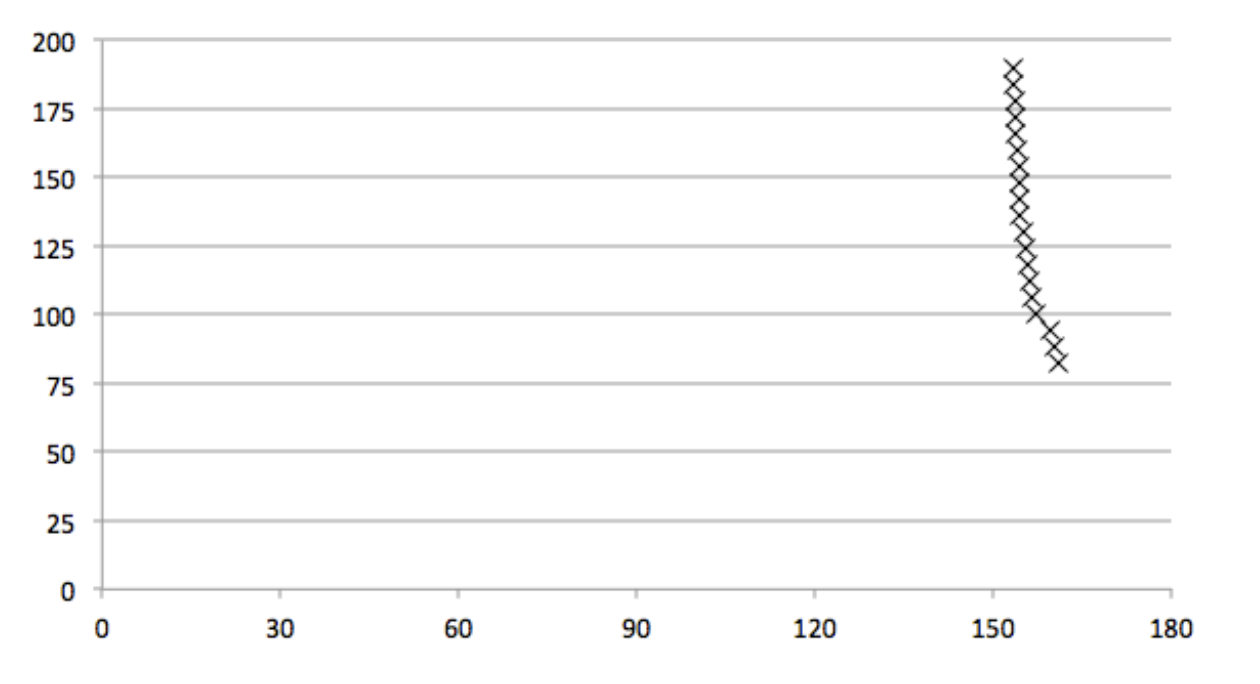
\includegraphics[ height=8cm]{Dissertation/images/base_line/SNPR_lit.png}
\caption{62 Sniper homogeneous transaction diagram with 100 price equilibrium from \cite{BSE_lit}} 
\end{figure} 
\FloatBarrier

\begin{figure}[!htbp]
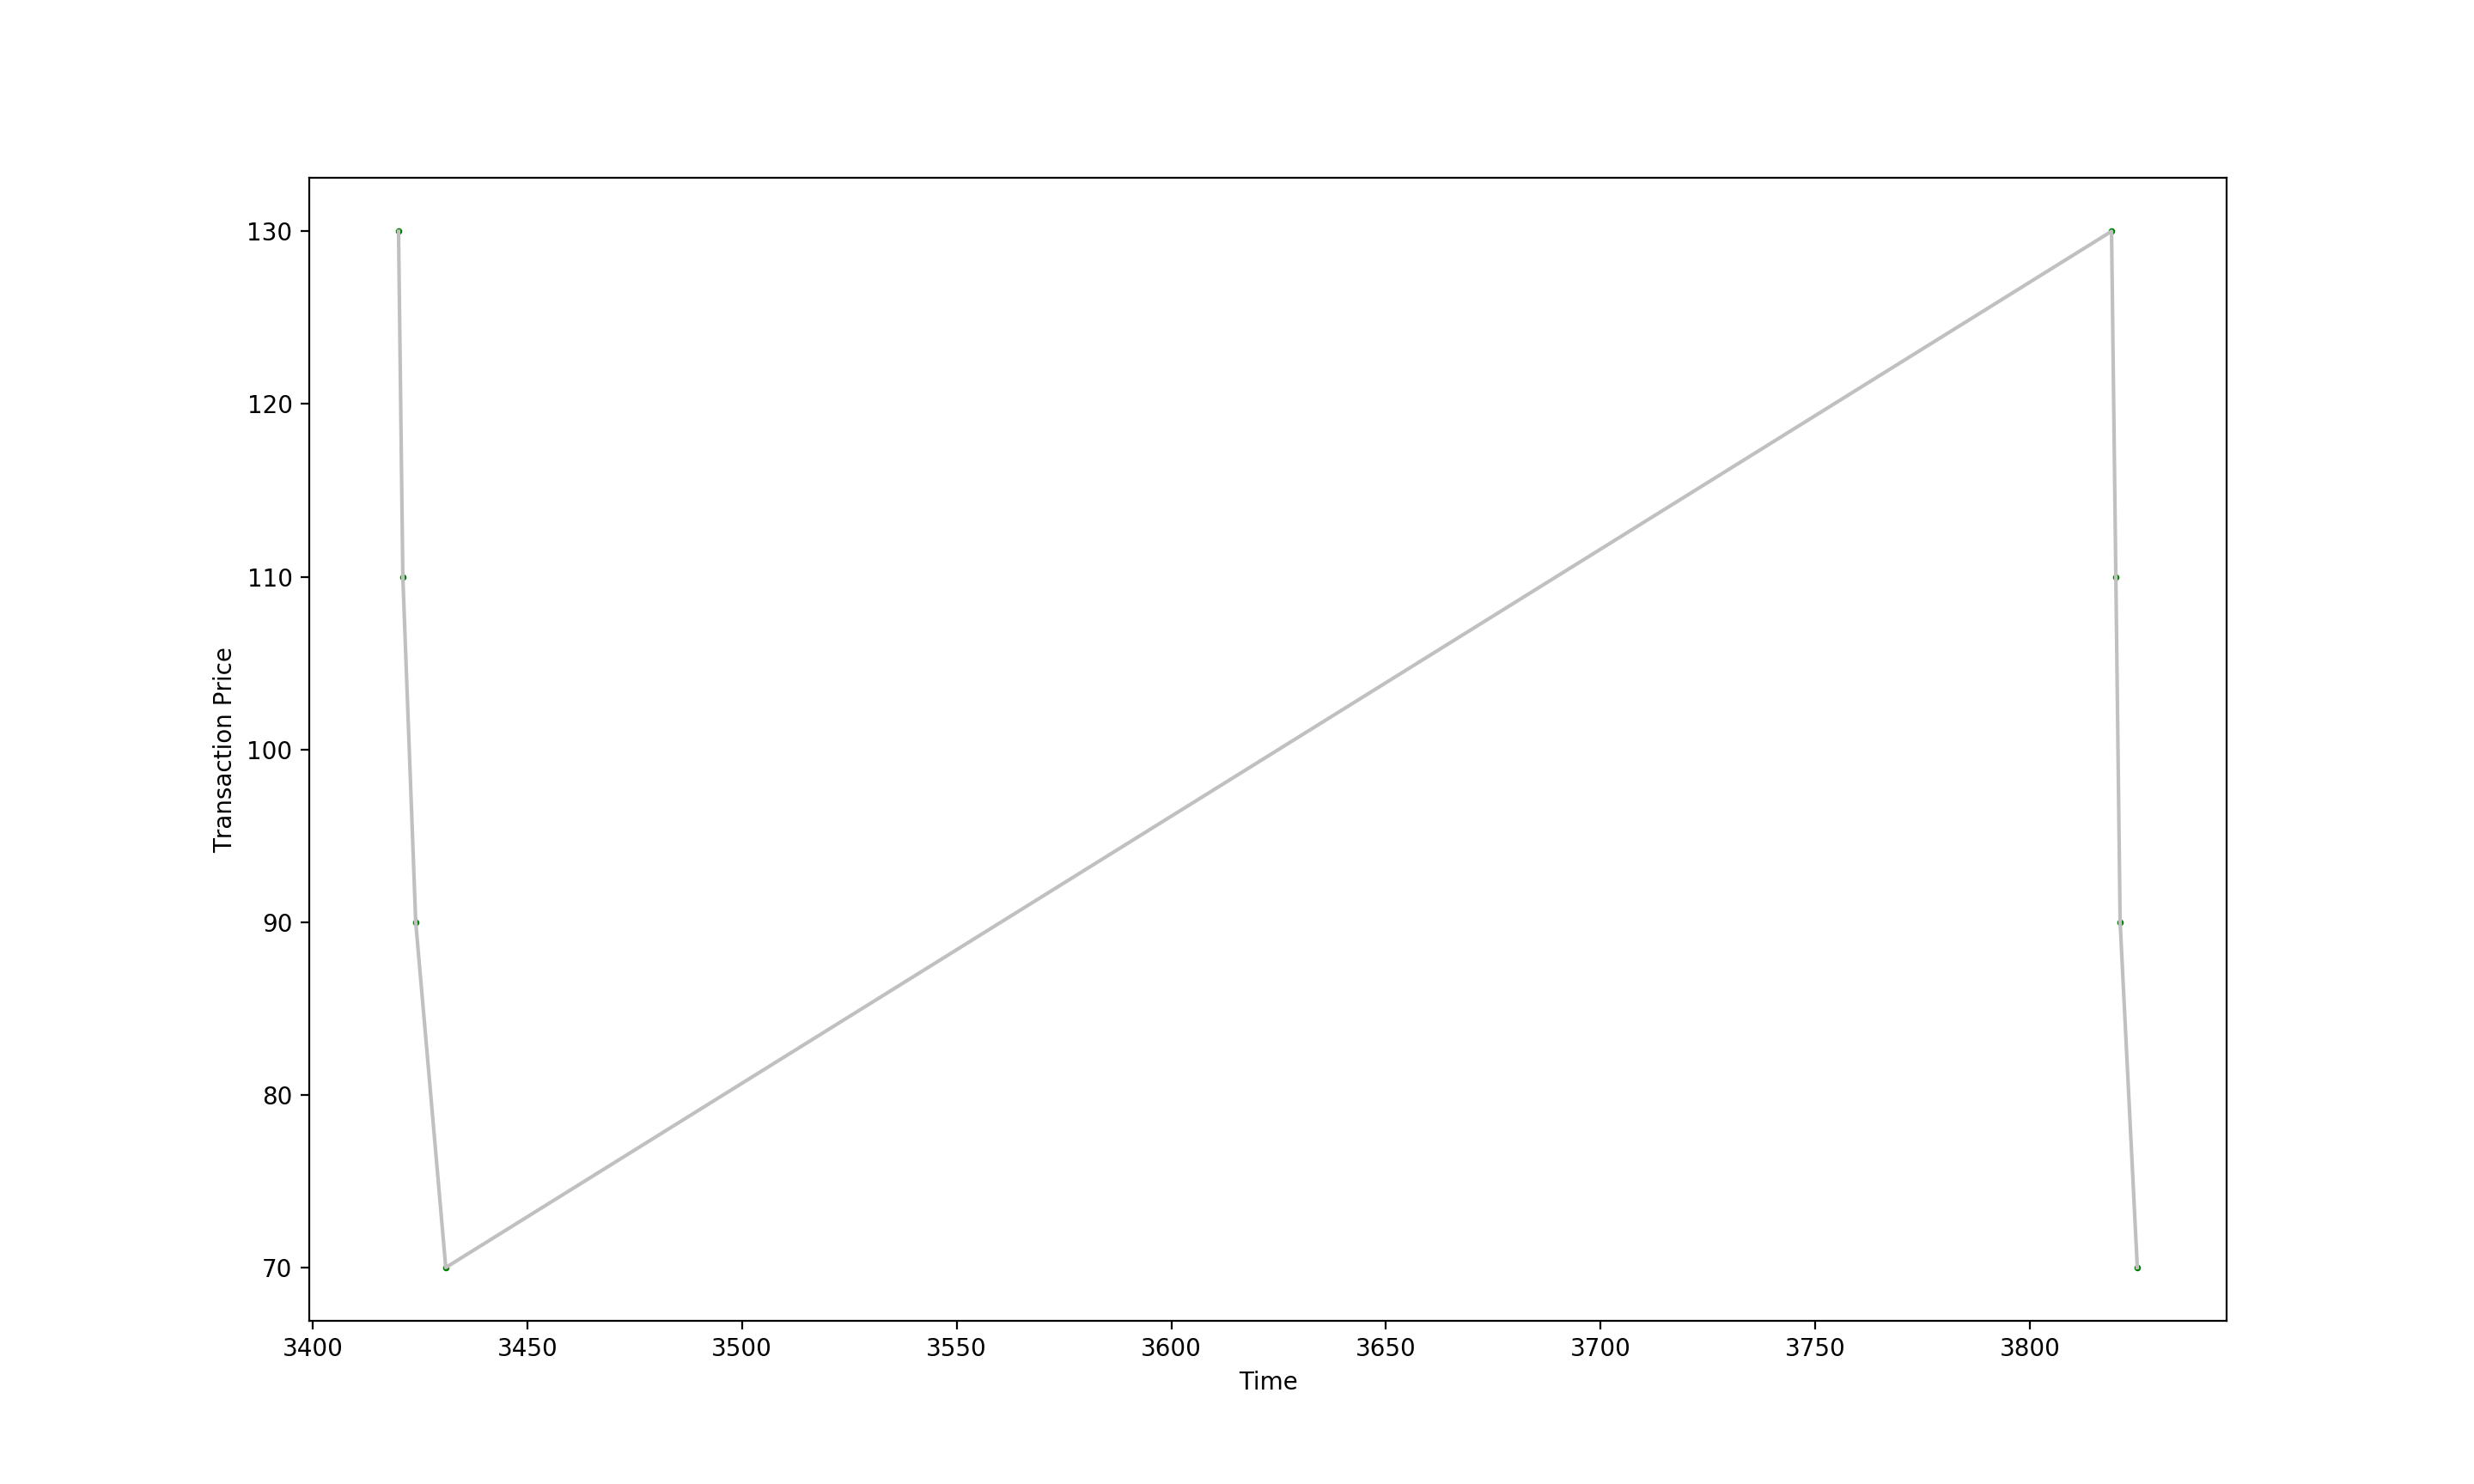
\includegraphics[ height=8cm]{Dissertation/images/base_line/sniper.png}
\caption{62 Sniper homogeneous transaction diagram with 100 price equilibrium from original BSE code} 
\end{figure} 
\FloatBarrier

\subsection{ZI-C}
ZI-C or Zero-Intelligence Constrained is another agent implemented in the original BSE. An expected behaviour of a market consisting of only ZI-C agents is a non-convergence transaction price. This is consistent with the Figure 4.2 below where at the end of the transaction period, the price does not converge to the equilibrium but instead exhibit a volatile price changes over the time period. 

\begin{figure}[h]
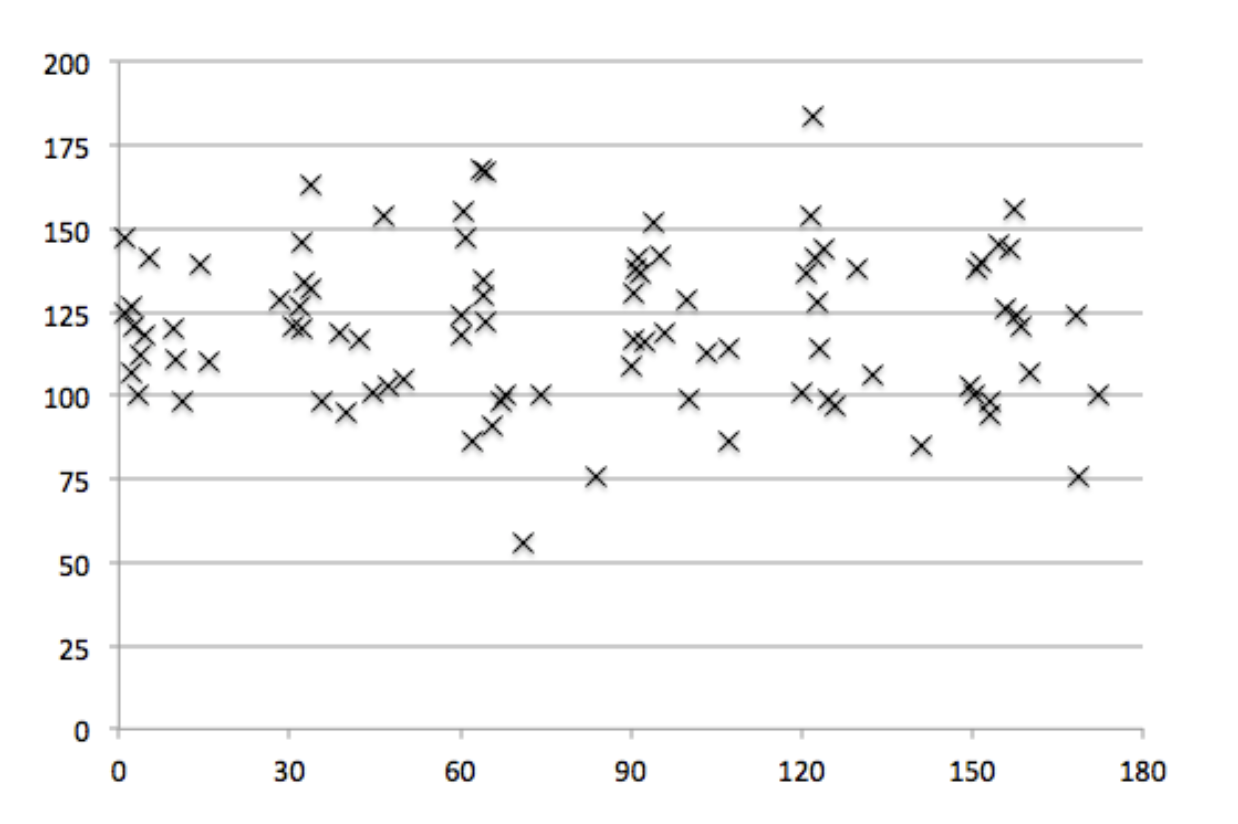
\includegraphics[ height=8cm]{Dissertation/images/base_line/zic_lit.png}
\caption{62 ZI-C homogeneous transaction diagram with 100 price equilibrium from \cite{BSE_lit}} 
\end{figure} 
\FloatBarrier

\begin{figure}[!htbp]
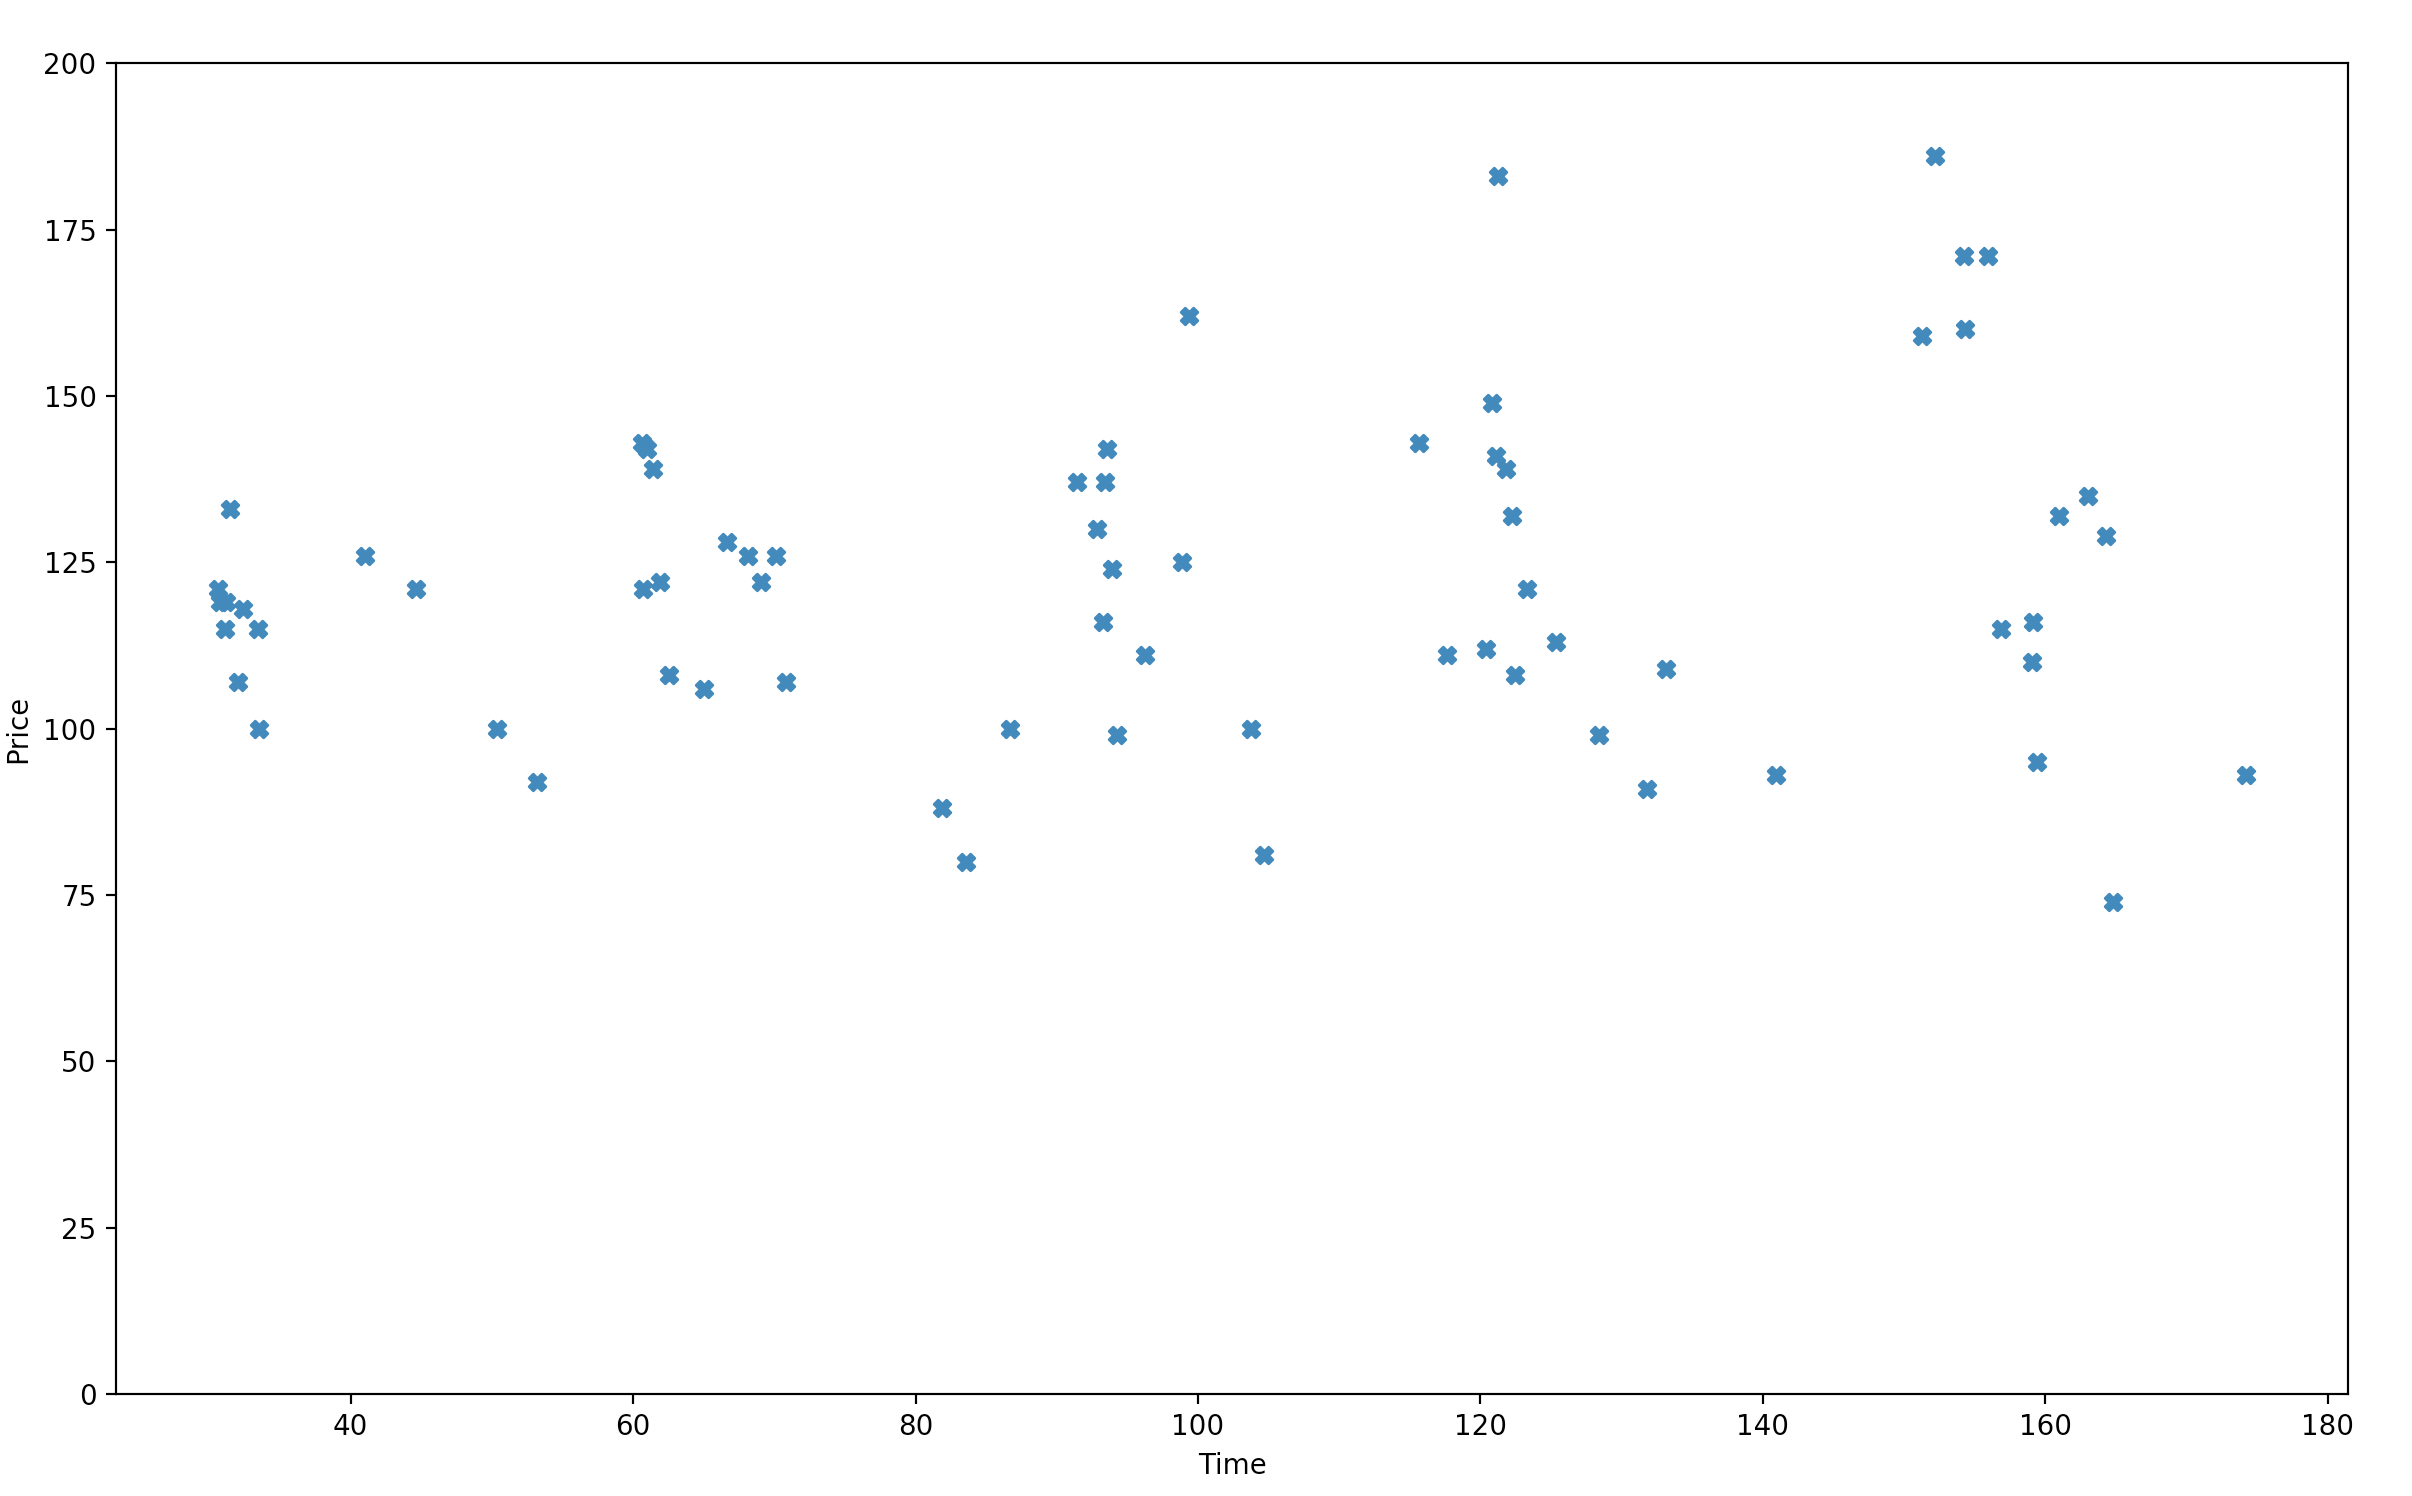
\includegraphics[ height=8cm]{Dissertation/images/base_line/ZIC.png}
\caption{62 ZI-C homogeneous transaction diagram with 100 price equilibrium from BSE original code} 
\end{figure} 
\FloatBarrier


\subsection{ZI-P}
ZI-P or Zero-Intelligence Plus is the agent that, in a homogeneous market, does produce the transaction price which converges to the equilibrium. A market of ZI-P agents is a good indicator to test the market structure and functions. In the Figure 4.3 below, the transaction price first fluctuates early in the transaction period but then converges towards 70 in the end of the session.  

\begin{figure}[h]
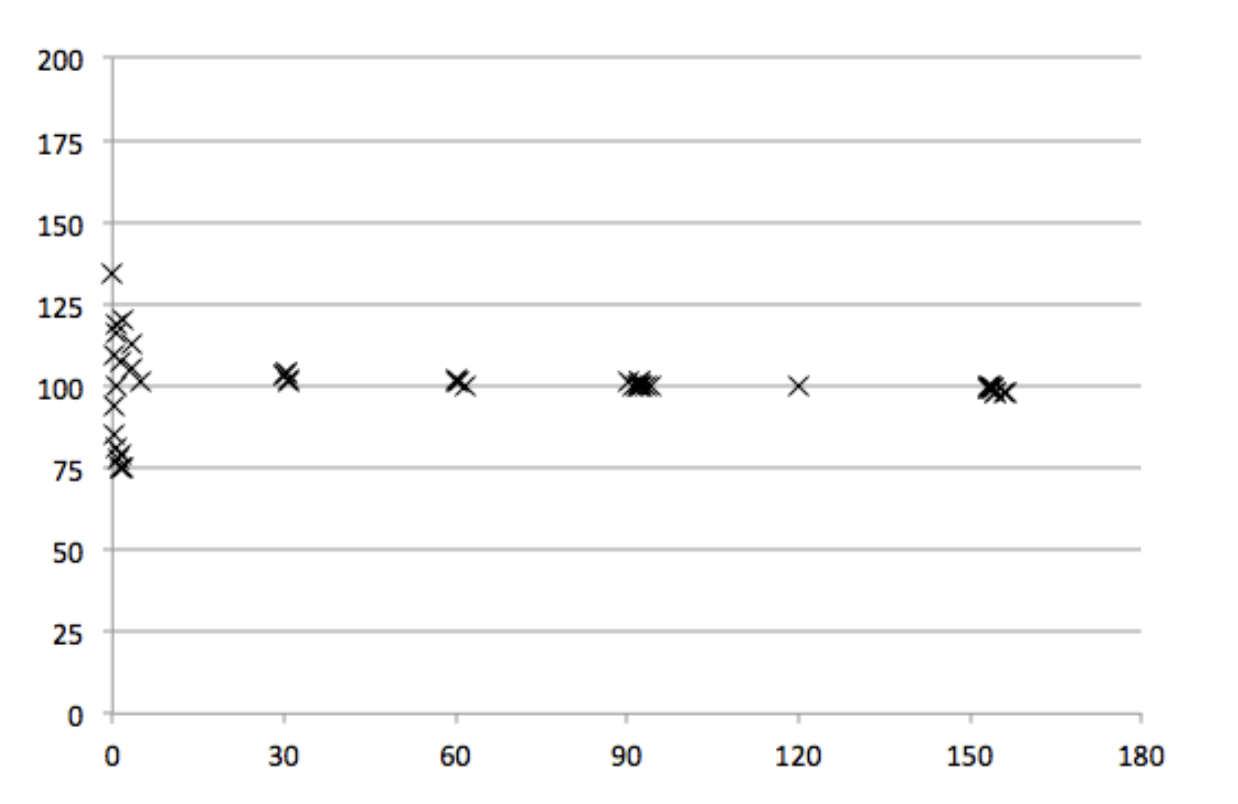
\includegraphics[ height=8cm]{Dissertation/images/base_line/zip_lit.png}
\caption{62 ZI-P homogeneous transaction diagram with 100 price equilibrium from \cite{BSE_lit}} 
\end{figure} 
\FloatBarrier

\begin{figure}[h]
\includegraphics[ height=8cm]{Dissertation/images/base_line/zip.png}
\caption{62 ZI-P homogeneous transaction diagram with 100 price equilibrium from original BSE code} 
\end{figure} 
\FloatBarrier

\section{Results after implementing complex order types} 
These results are from tests ran with the same configuration as the Base Line tests. These tests are ran after the LOB has been re-configured to be able to accept more than one type of order (Market Order as well as Limit Order) in addition to more than one quantity. The tests are ran with the same time step as the original BSE. 

\begin{table}[h]
\centering
\begin{tabular}{ |m||p{4cm}|p{4cm}|} 
\hline
\textbf{Agents}& \textbf{Base Line Smith's alpha value}& \textbf{Smith's alpha value} \\
\hline
\hline
Kaplan's Sniper & 49.73  & 49.51 \\ 
\hline
ZI-C  & 63.5 & 64.3\\ 
\hline
ZI-P & 24.8 & 22.4 \\ 
\hline
\end{tabular}
\caption{Smith's alpha value after implementing complex order types}  
\end{table}
\FloatBarrier


\subsection{Kaplan's Sniper}
As expected, the Sniper only submits orders near the end of the session, which makes the first transactions only appear after $t = 160$.  
\begin{figure}[h]
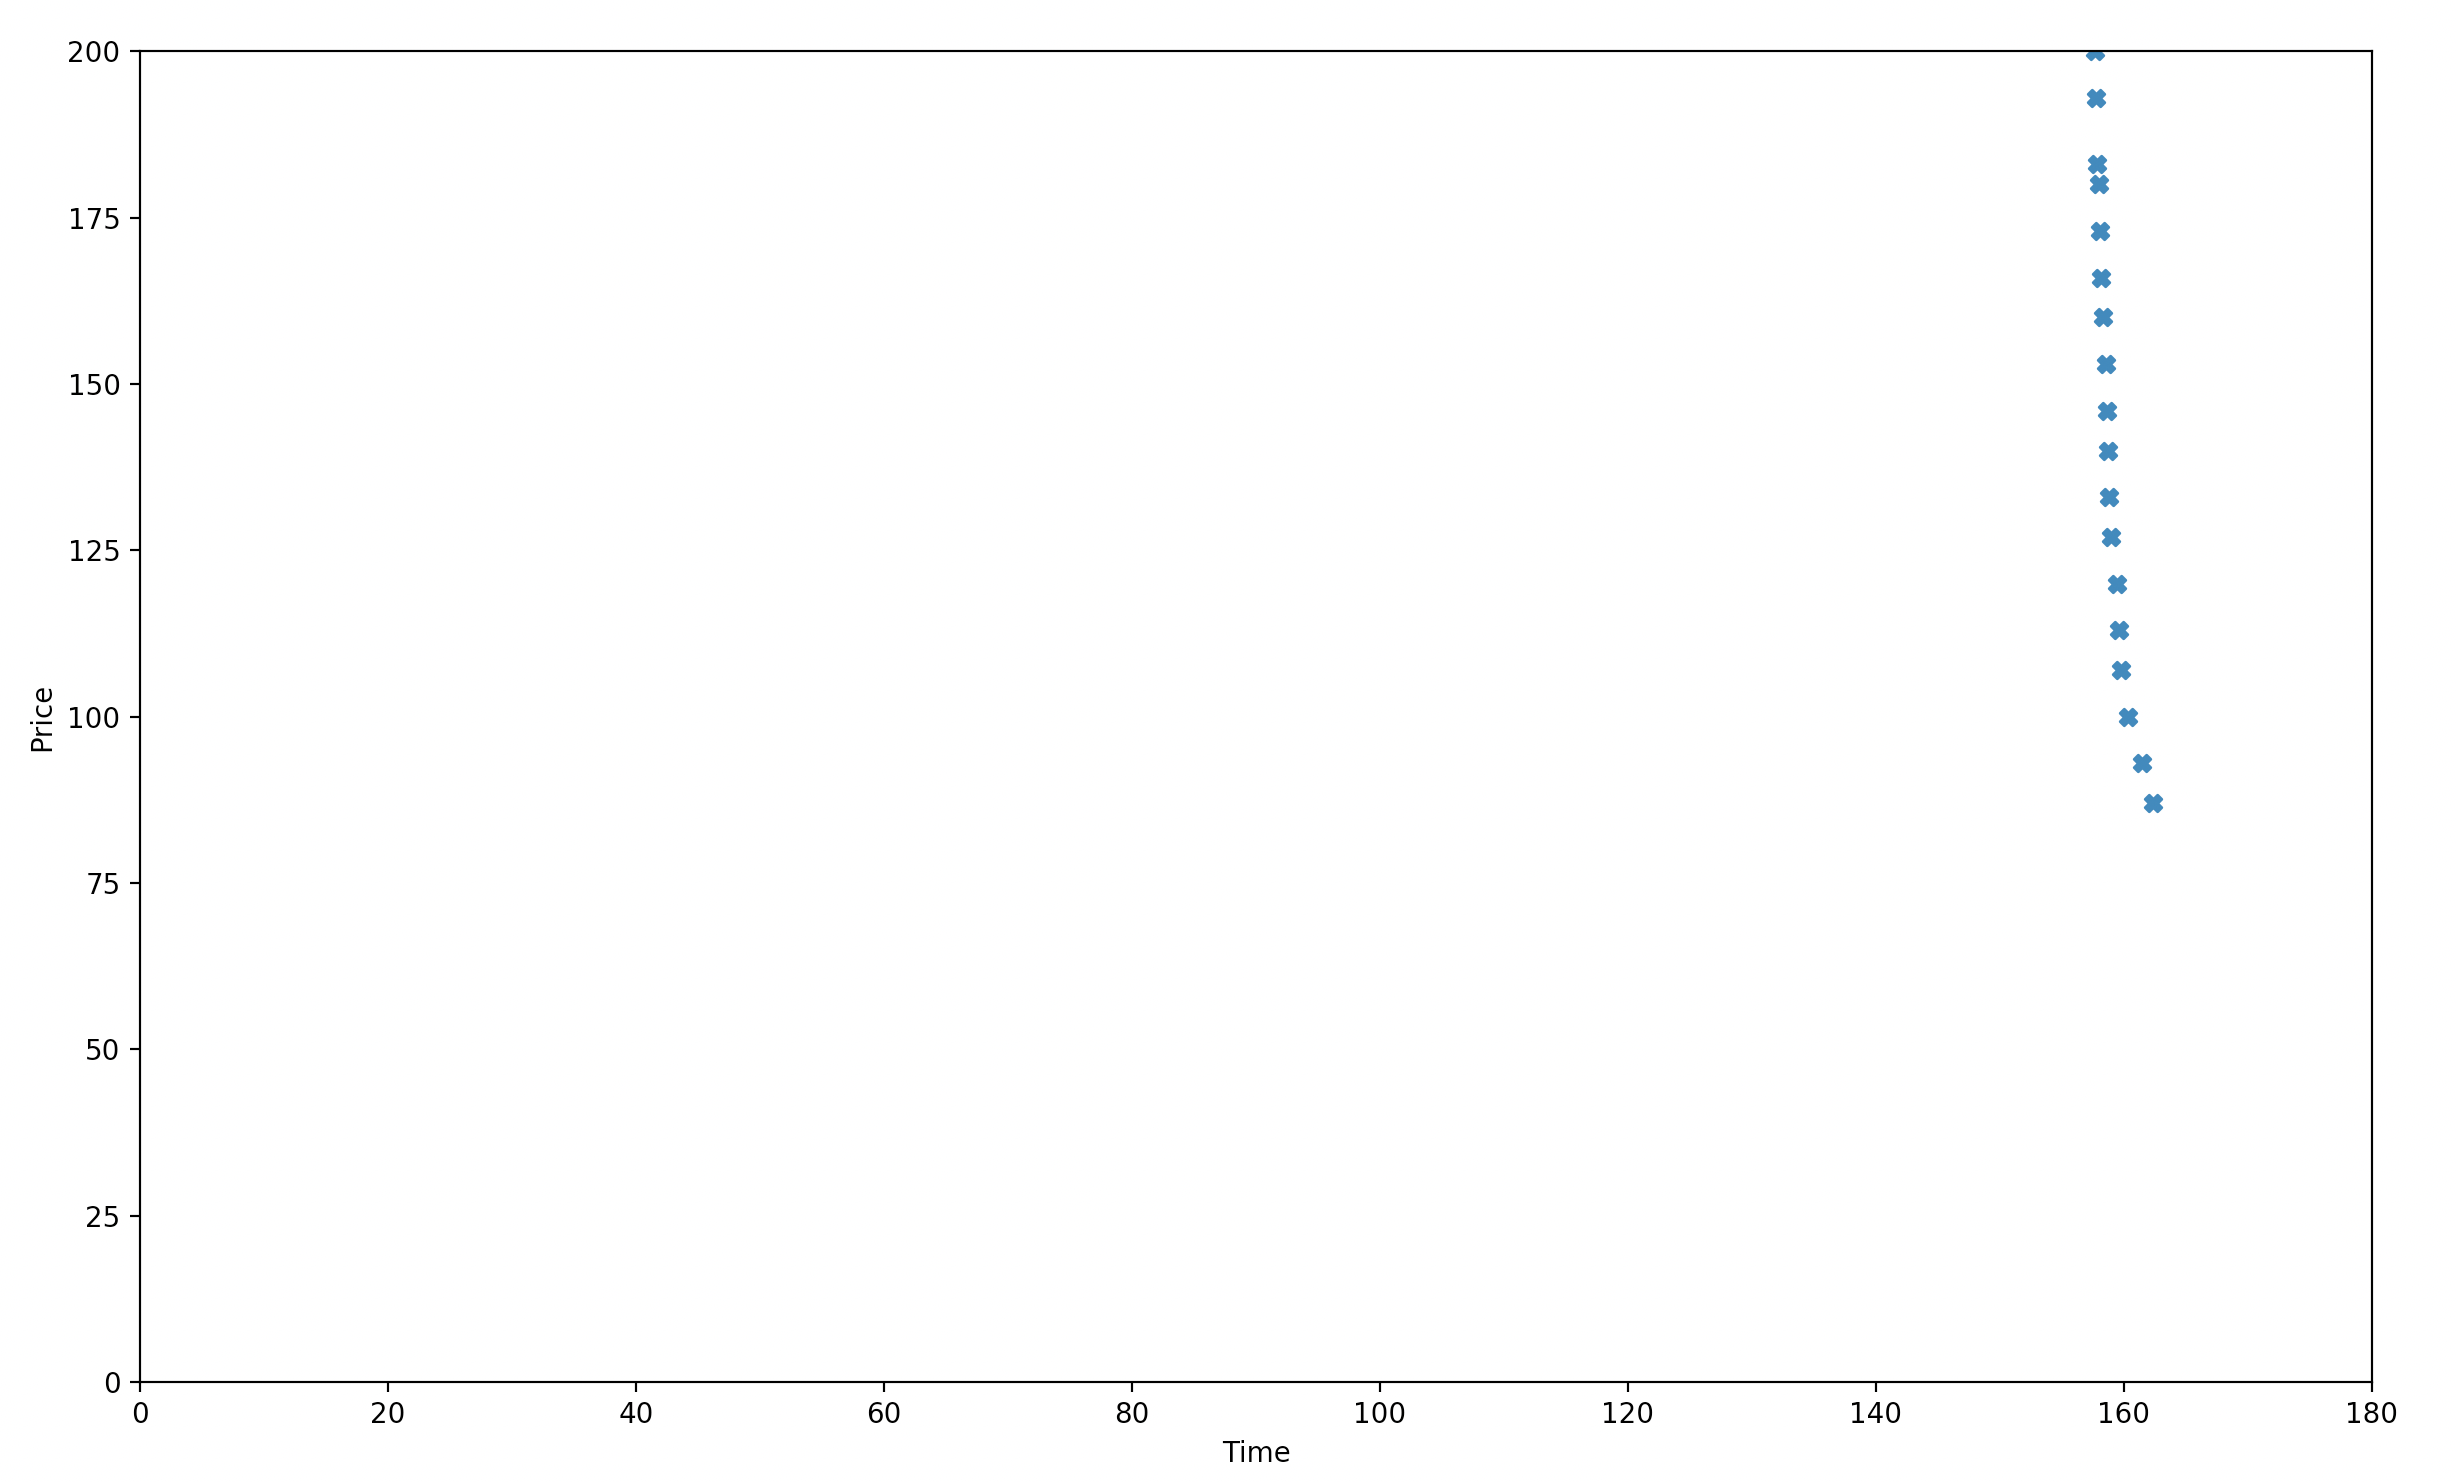
\includegraphics[ height=7cm]{Dissertation/images/change1/snpr.png}
\caption{62 Sniper agents homogeneous market transaction diagram with 100 price equilibrium from complex order types implementation} 
\end{figure} 
\FloatBarrier

\subsection{ZI-C}
ZIC's behaviour in the new LOB is still similar to the one ran in the original BSE. The transaction price does not converge in any period of the session. 

\begin{figure}[h]
\includegraphics[ height=8cm]{Dissertation/images/change1/zic.png}
\caption{62 ZI-C agents homogeneous market transaction diagram with 100 price equilibrium from complex order types implementation} 
\end{figure} 
\FloatBarrier

\subsection{ZI-P}
ZIP illustrates a convergence to the 100 equilibrium as expected. 

\begin{figure}[h]
\includegraphics[ height=8cm]{Dissertation/images/change1/zip.png}
\caption{62 ZI-P agents homogeneous market transaction diagram with 100 price equilibrium from complex order types implementation} 
\end{figure} 
\FloatBarrier

\section{Results after implementing McG action step} 
This section illustrate the results with same test configurations on the BSE with McG action step. The McG action step is similar to the BSE except that it does not divide the individual time-step by the number of buyers and sellers then select them randomly. The McG time step loops through every trader in each time-step, allowing the trader to act in all the time steps. The time period selected is 11,160 which is equivalent to the 180 time step in original BSE time-step. In addition, the interval is changed to be 10\% of the time-step for the customer order (price assignments) which is 1,860 in the McG and 30 in the original BSE. The results of the tests are illustrated below. 

\begin{table}[h]
\centering
\begin{tabular}{ |m||p{4cm}|p{4cm}|p{4cm}|} 
\hline
\textbf{Agents}& \textbf{Base Line Smith's alpha value} & \textbf{Smith's alpha value for section 4.2} & \textbf{Smith's alpha value} \\
\hline
\hline
Kaplan's Sniper & 49.73  & 49.51 & 50.1 \\ 
\hline
ZI-C & 63.5 & 64.3 & 67.3\\ 
\hline
ZI-P & 24.8 & 22.4 & 25.4 \\ 
\hline
\end{tabular}
\caption{Smith's alpha value after implementing McG action step}  
\end{table}
\FloatBarrier

\subsection{Kaplan's Sniper}
As expected, the Sniper only submits orders near the end of the session, which makes the first transactions only appear after $t = 9000$. However, figure 4.10 suggests that the behaviour of the Sniper agent is not entirely the same as there are similar transactions from the agents submitting two sets of similar orders in the end of the period. This is partly because the gap between 9,000 - 11,160 is much higher than 160 - 180 in previous experiments. Therefore, the agents have time to submit two different sets of orders. This suggests that there needs to be some adaptation to the agent's values in order to retain the behaviour it has in the base line experiment. 

\begin{figure}[h]
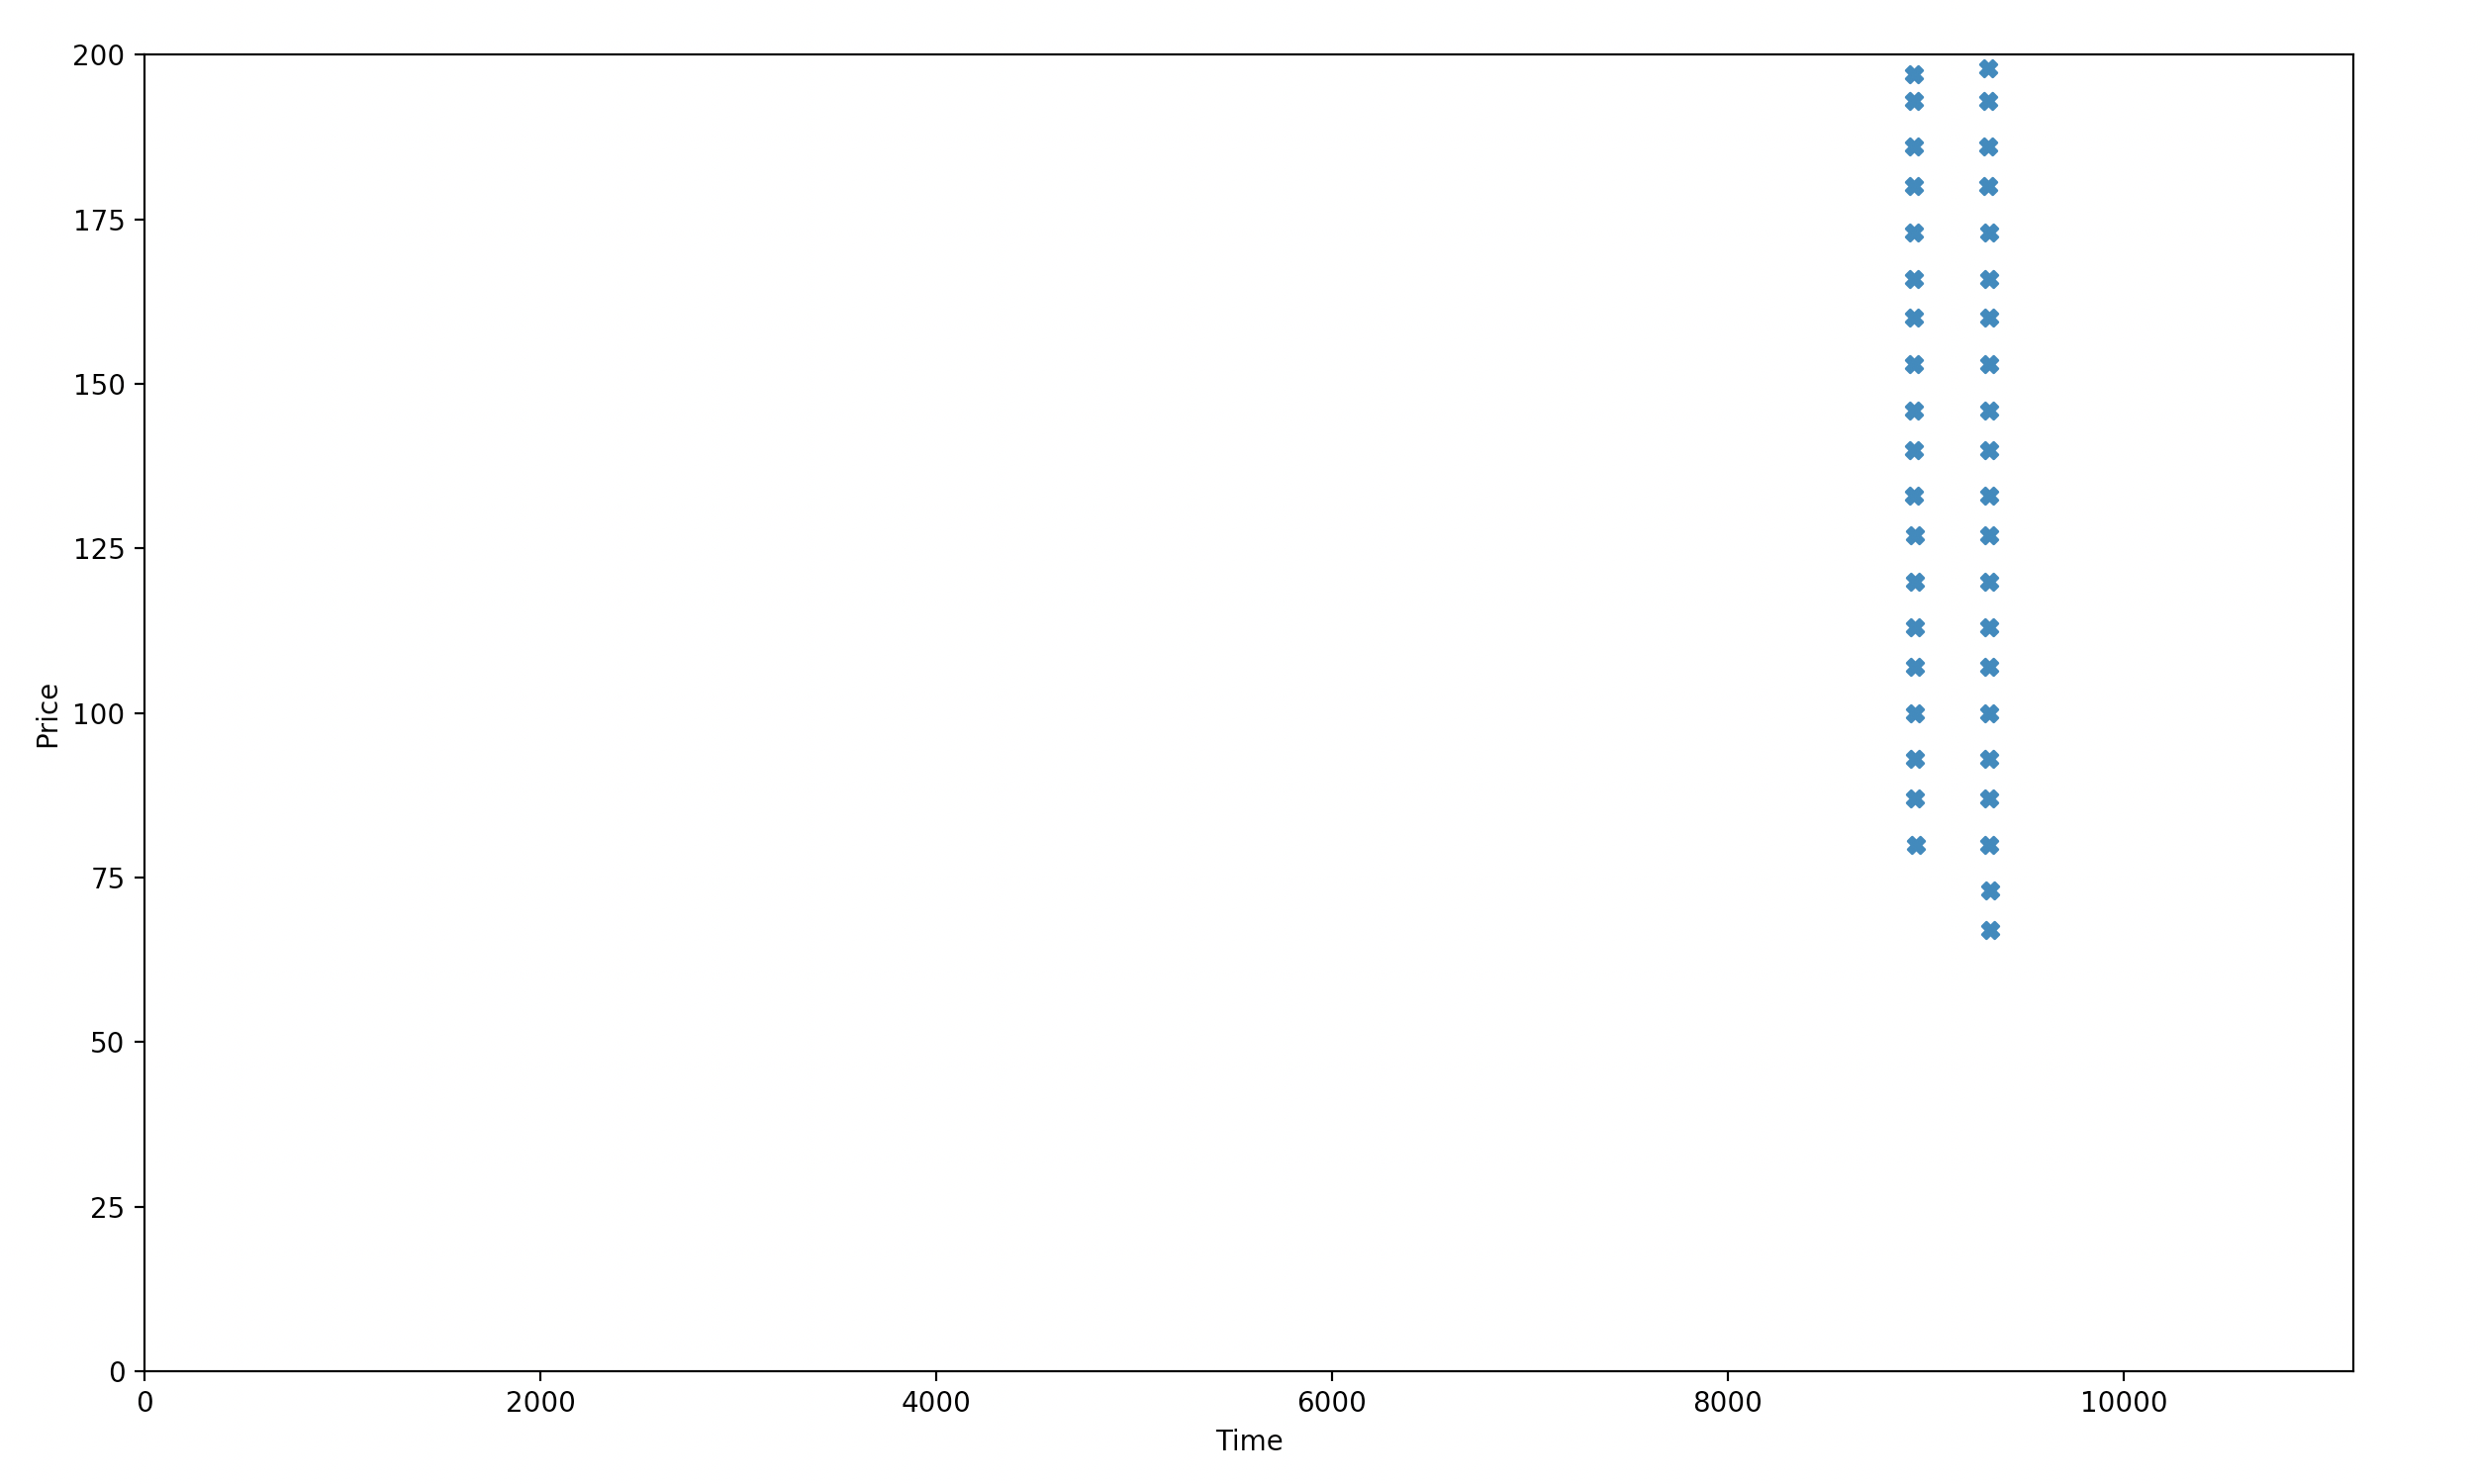
\includegraphics[ height=8cm]{Dissertation/images/snpr_adapted/2lines.png}
\caption{62 Sniper agents homogeneous market transaction diagram with 100 price equilibrium from complex order types implementation} 
\end{figure} 
\FloatBarrier

After reducing the lurk threshold from 0.2 to 0.1, the agent behaviour now matches the base line results. 

\begin{figure}[h]
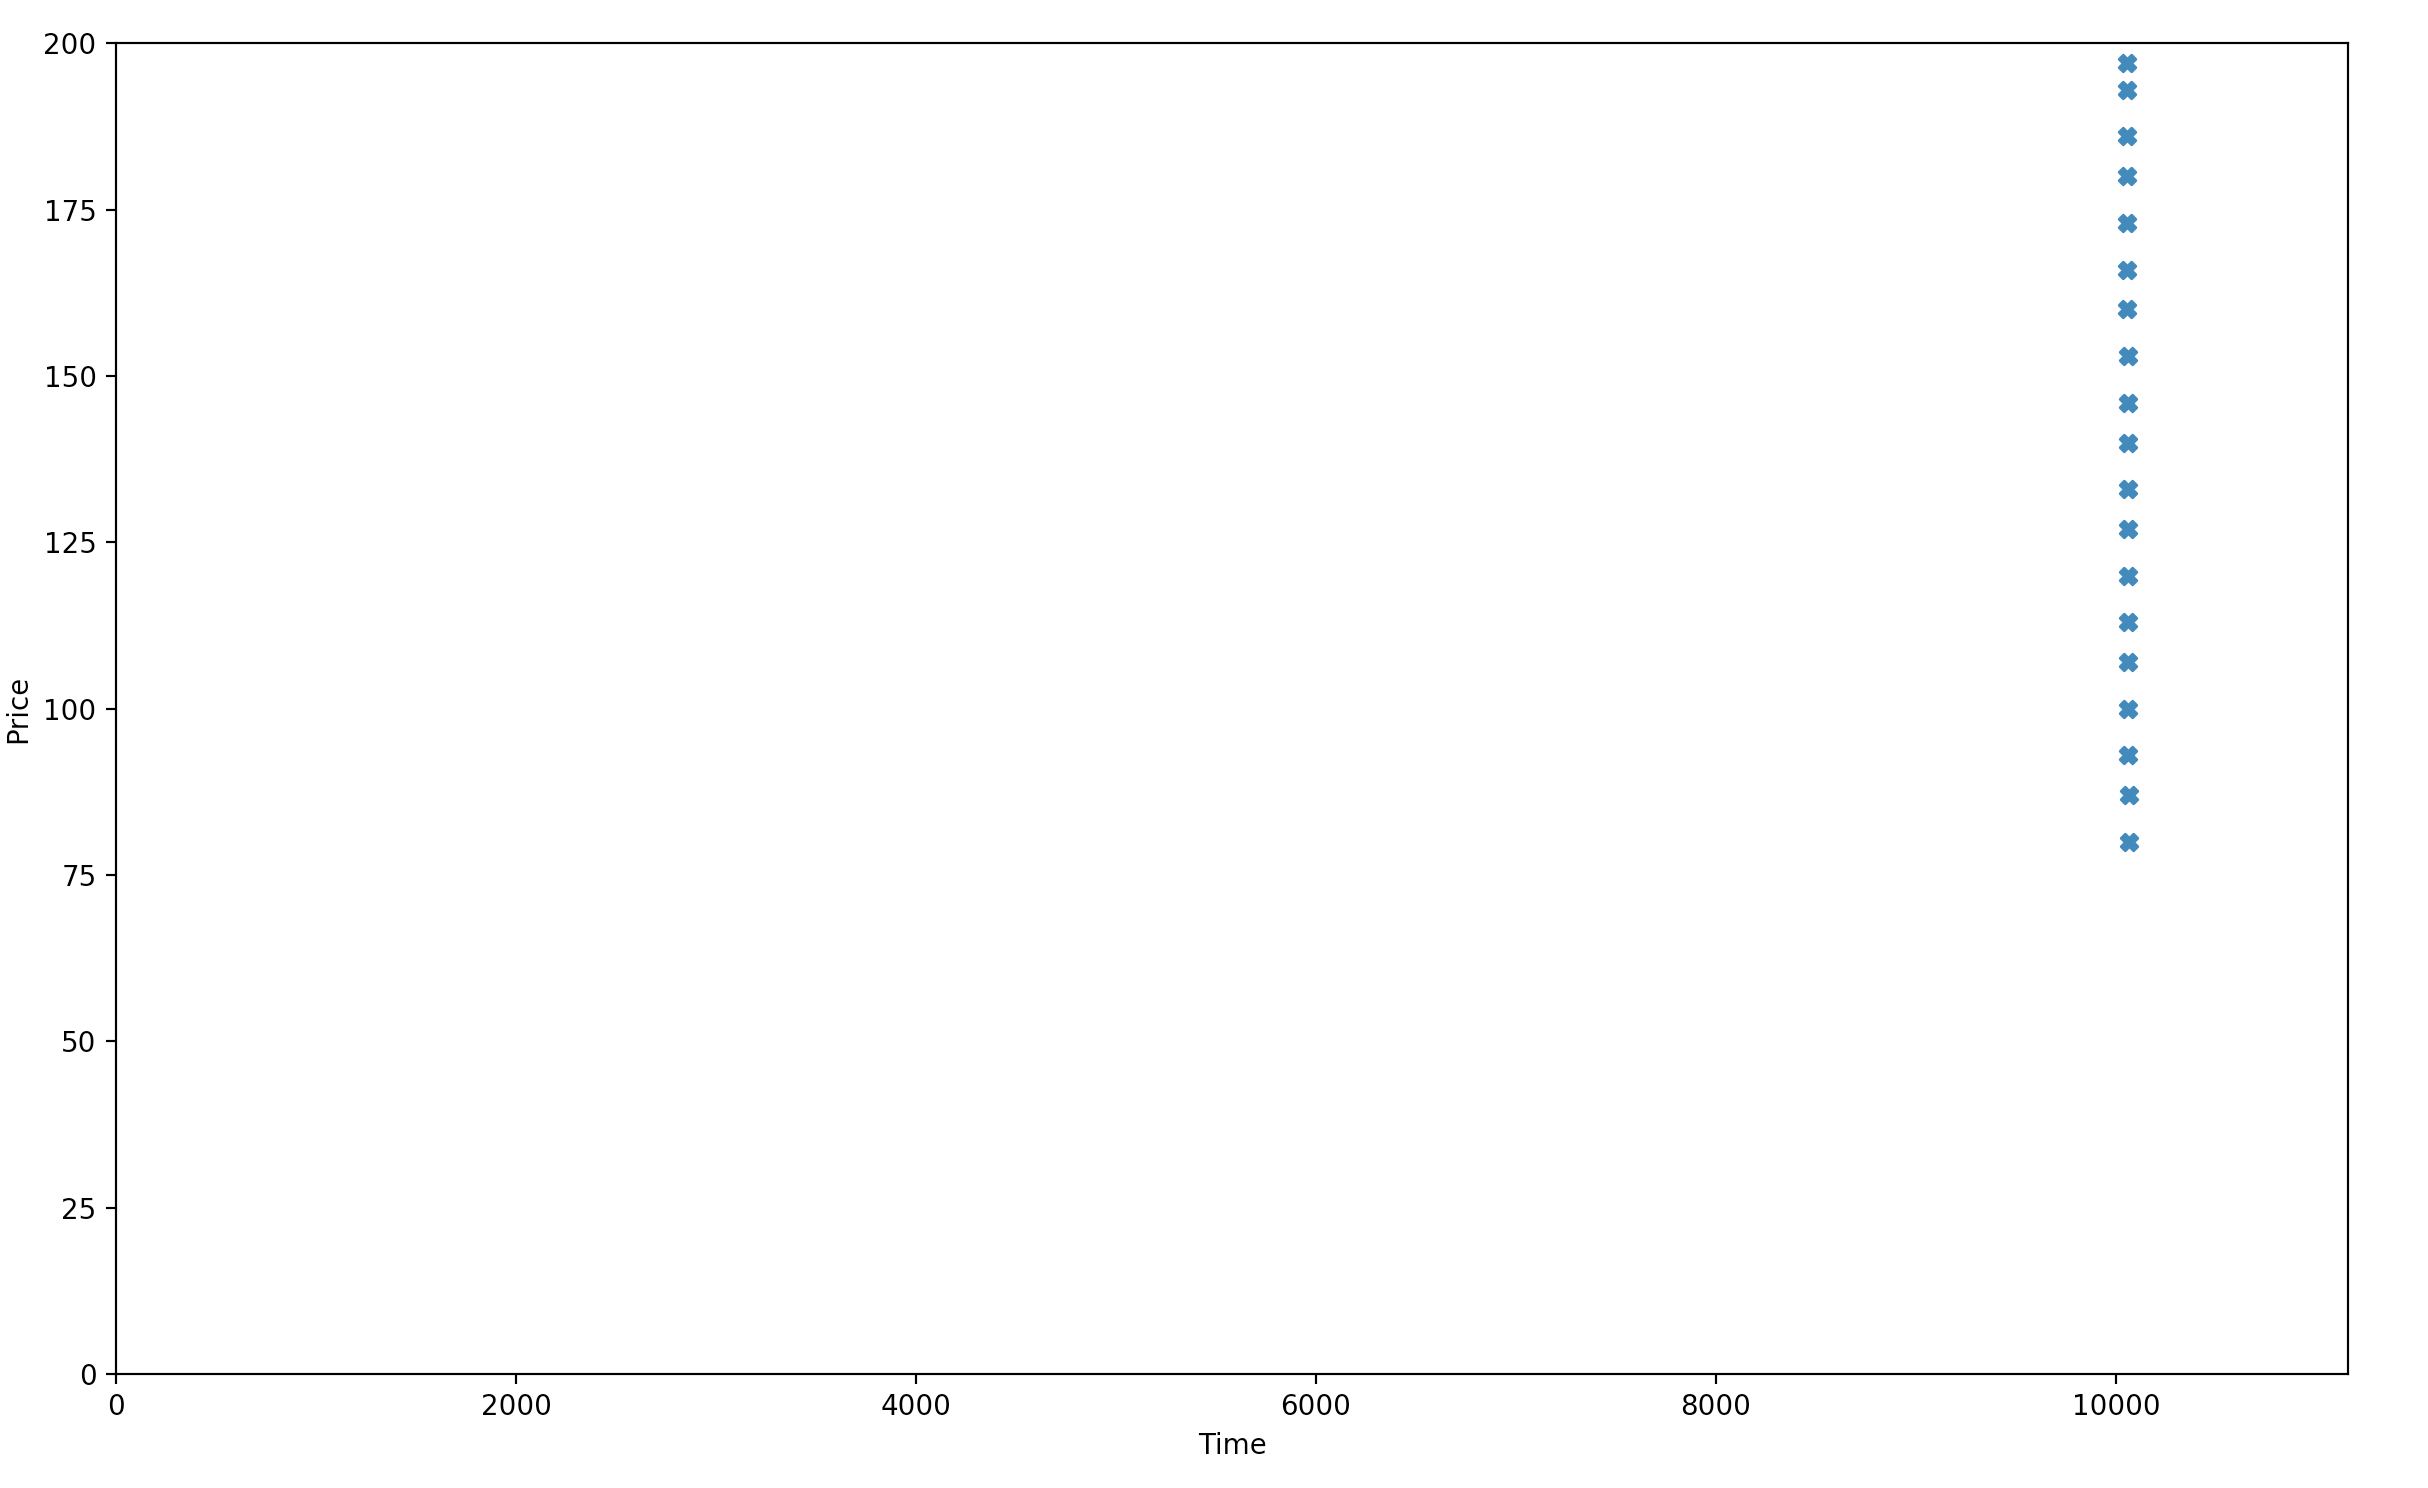
\includegraphics[ height=8cm]{Dissertation/images/snpr_adapted/adapted.png}
\caption{Adapted Sniper agent with Lurk threshold = 0.1} 
\end{figure} 
\FloatBarrier

\begin{figure}[h]
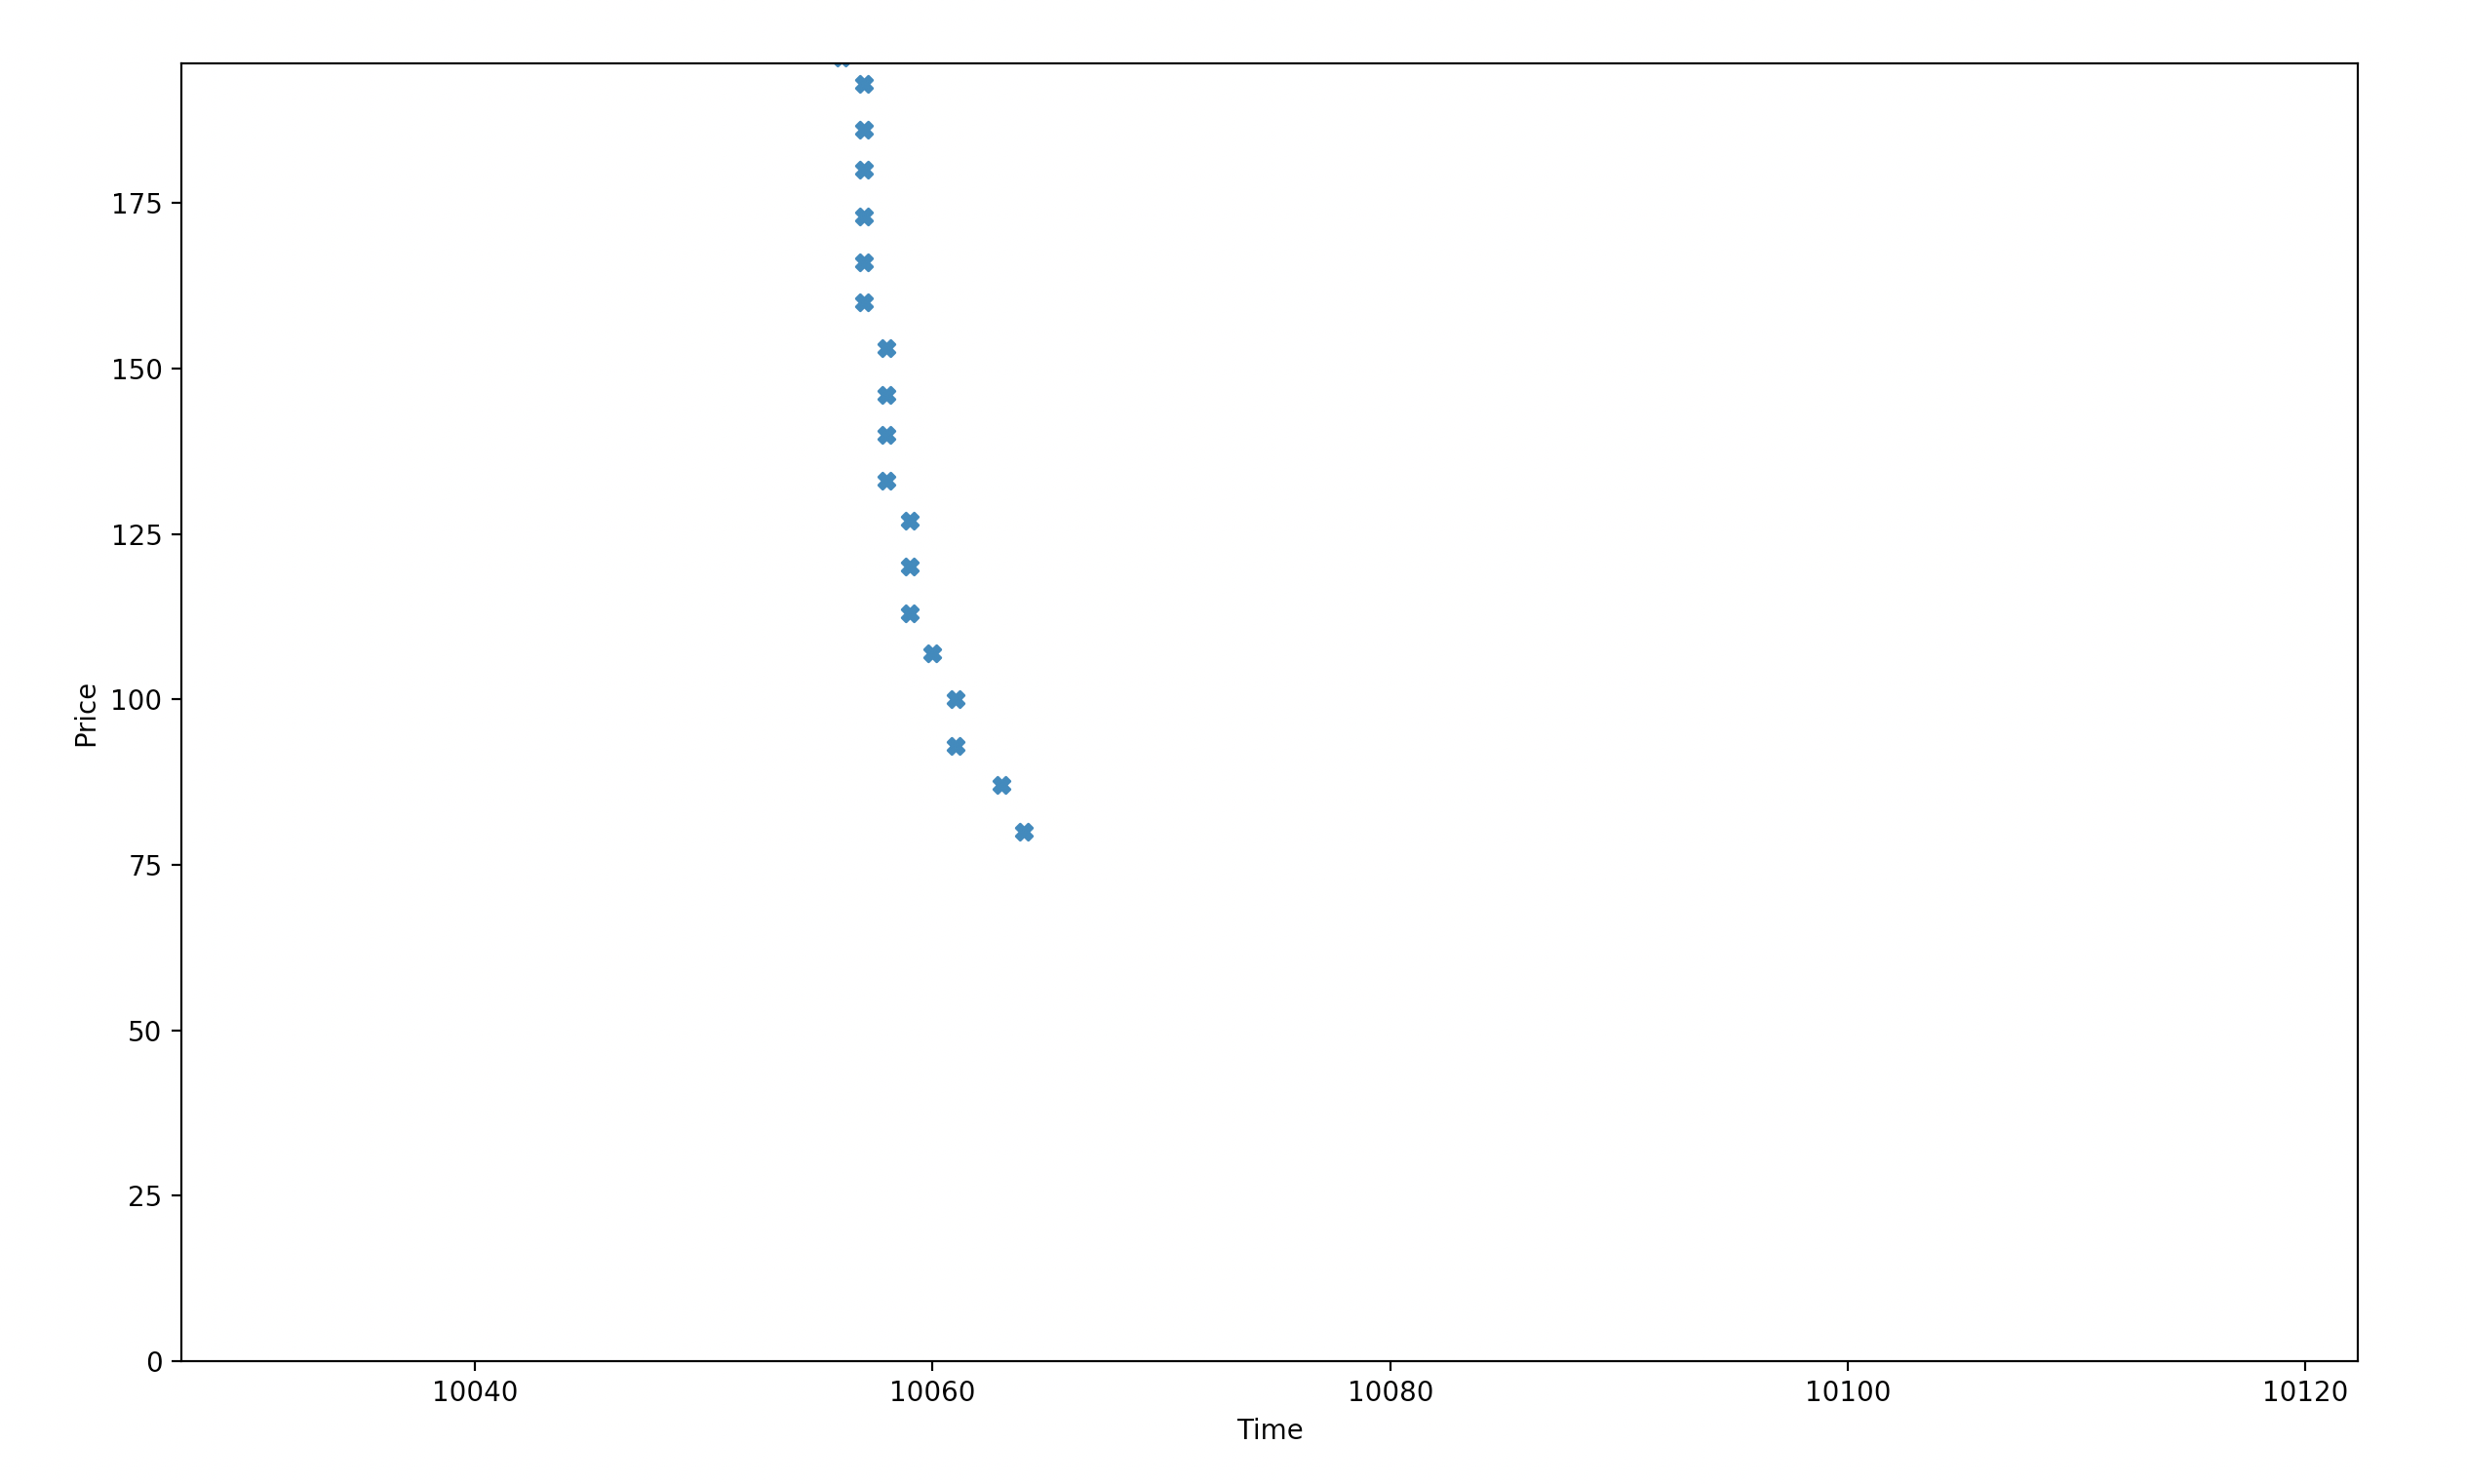
\includegraphics[ height=8cm]{Dissertation/images/snpr_adapted/zoom.png}
\caption{Zoomed-in graph of the figure 4.11} 
\end{figure} 
\FloatBarrier

% \begin{figure}[h]
%   \begin{subfigure}[b]{0.5\textwidth}
%     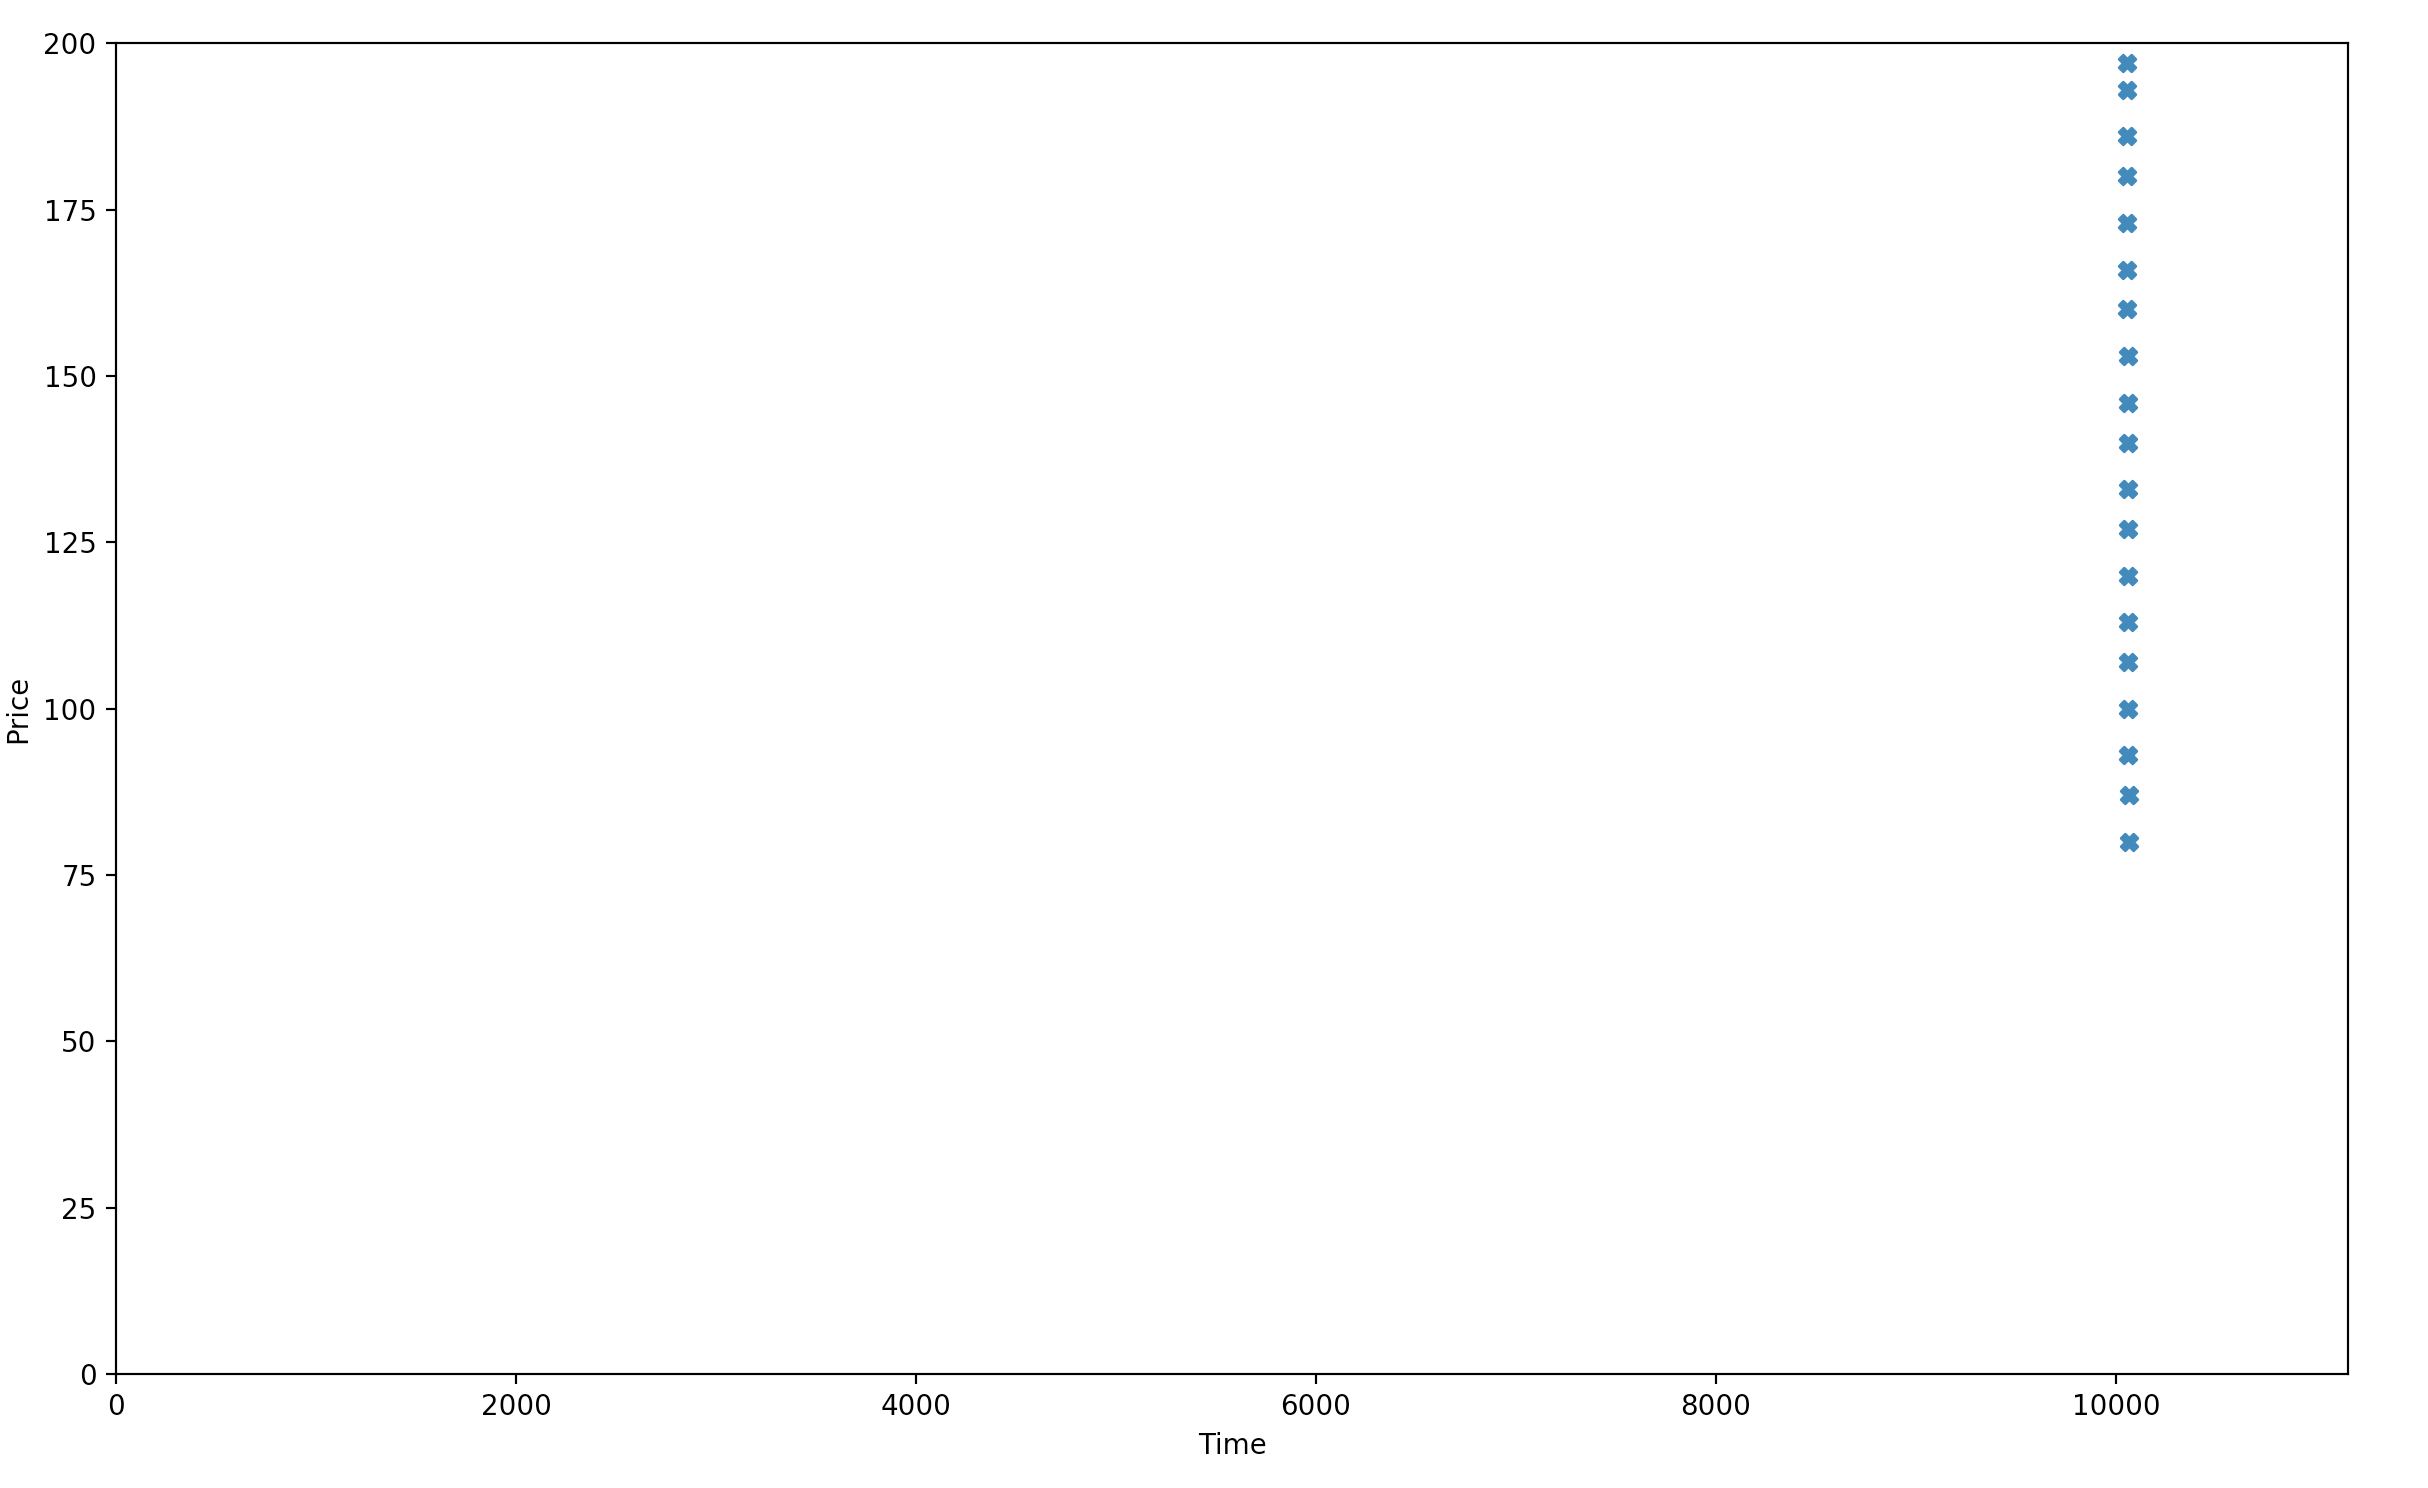
\includegraphics[width=7cm, height=8cm]{Dissertation/images/snpr_adapted/adapted.png}
%     \caption{Adapted Sniper agent with Lurk threshold = 0.1 }
%     \label{fig:1}
%   \end{subfigure}
%   %
%   \begin{subfigure}[b]{0.5\textwidth}
%     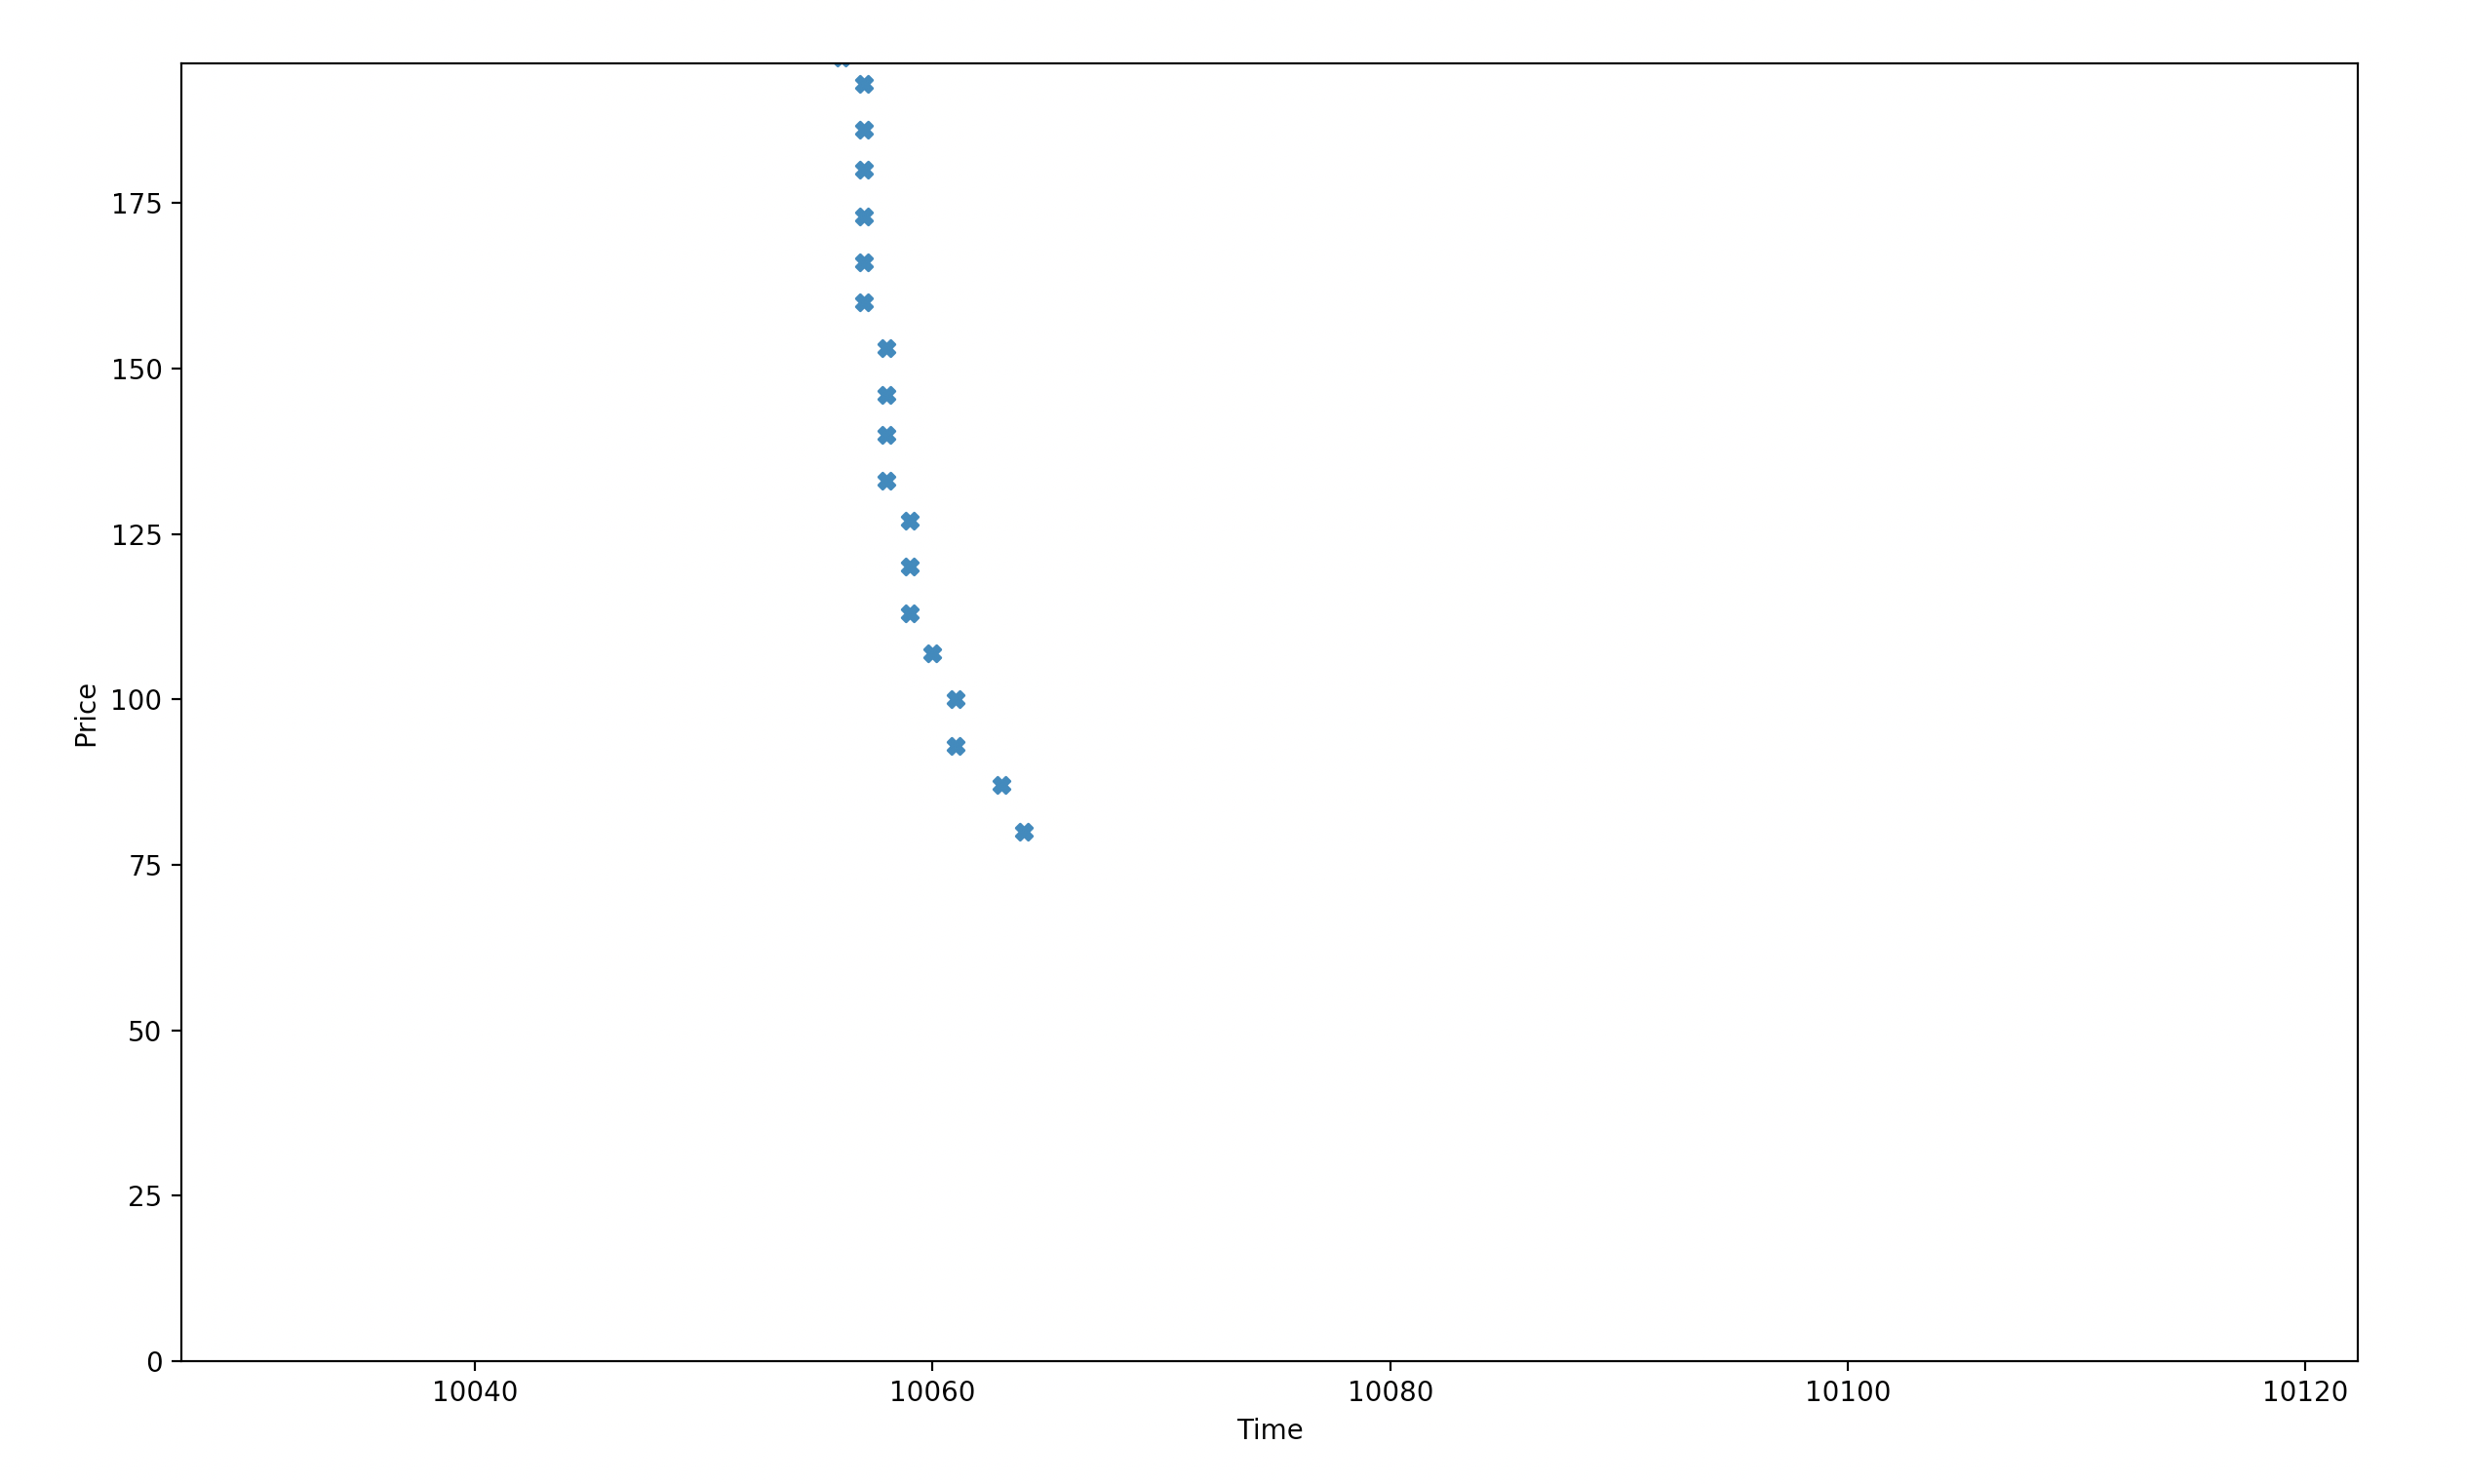
\includegraphics[width= 7cm, height=8cm]{Dissertation/images/snpr_adapted/zoom.png}
%     \caption{Zoomed-in graph of the left image}
%     \label{fig:2}
%   \end{subfigure}
% \end{figure}
% \FloatBarrier

\subsection{ZI-C}
ZIC's behaviour in the new LOB is still similar to the one ran in the original BSE. The transaction price does not converge in any period of the session.

\begin{figure}[h]
\includegraphics[ height=8cm]{Dissertation/images/change2/zic.png}
\caption{62 ZI-C agents homogeneous market transaction diagram with 100 price equilibrium from McG action step implementation}  
\end{figure} 
\FloatBarrier

\subsection{ZI-P}
In ZIP's case, the implementation and adaptation is much more complex. In the experiment, the results suggest that the probability of acting for ZI-P agent (implemented so that it is similar to the McG agents) play a huge role in the convergence of ZI-P equilibrium. The parameter $p_{zip}$ is the probability of acting of the ZI-P agent. The adaptation is very similar to how McG adapted the Oesch's agents to their model in which the Oesch's time system is very similar to that of BSE's. The figures below illustrate the examples of ZI-P converge in each probability. It can clearly be seen that as the probability decreases, the convergence will be better. In the 1 case, the ZI-P barely converges at all. However, as the probability in 0.5 and 0.25, the transaction price slowly converges near the equilibrium at 100. 

\begin{figure}[h]
  \begin{subfigure}[b]{0.5\textwidth}
    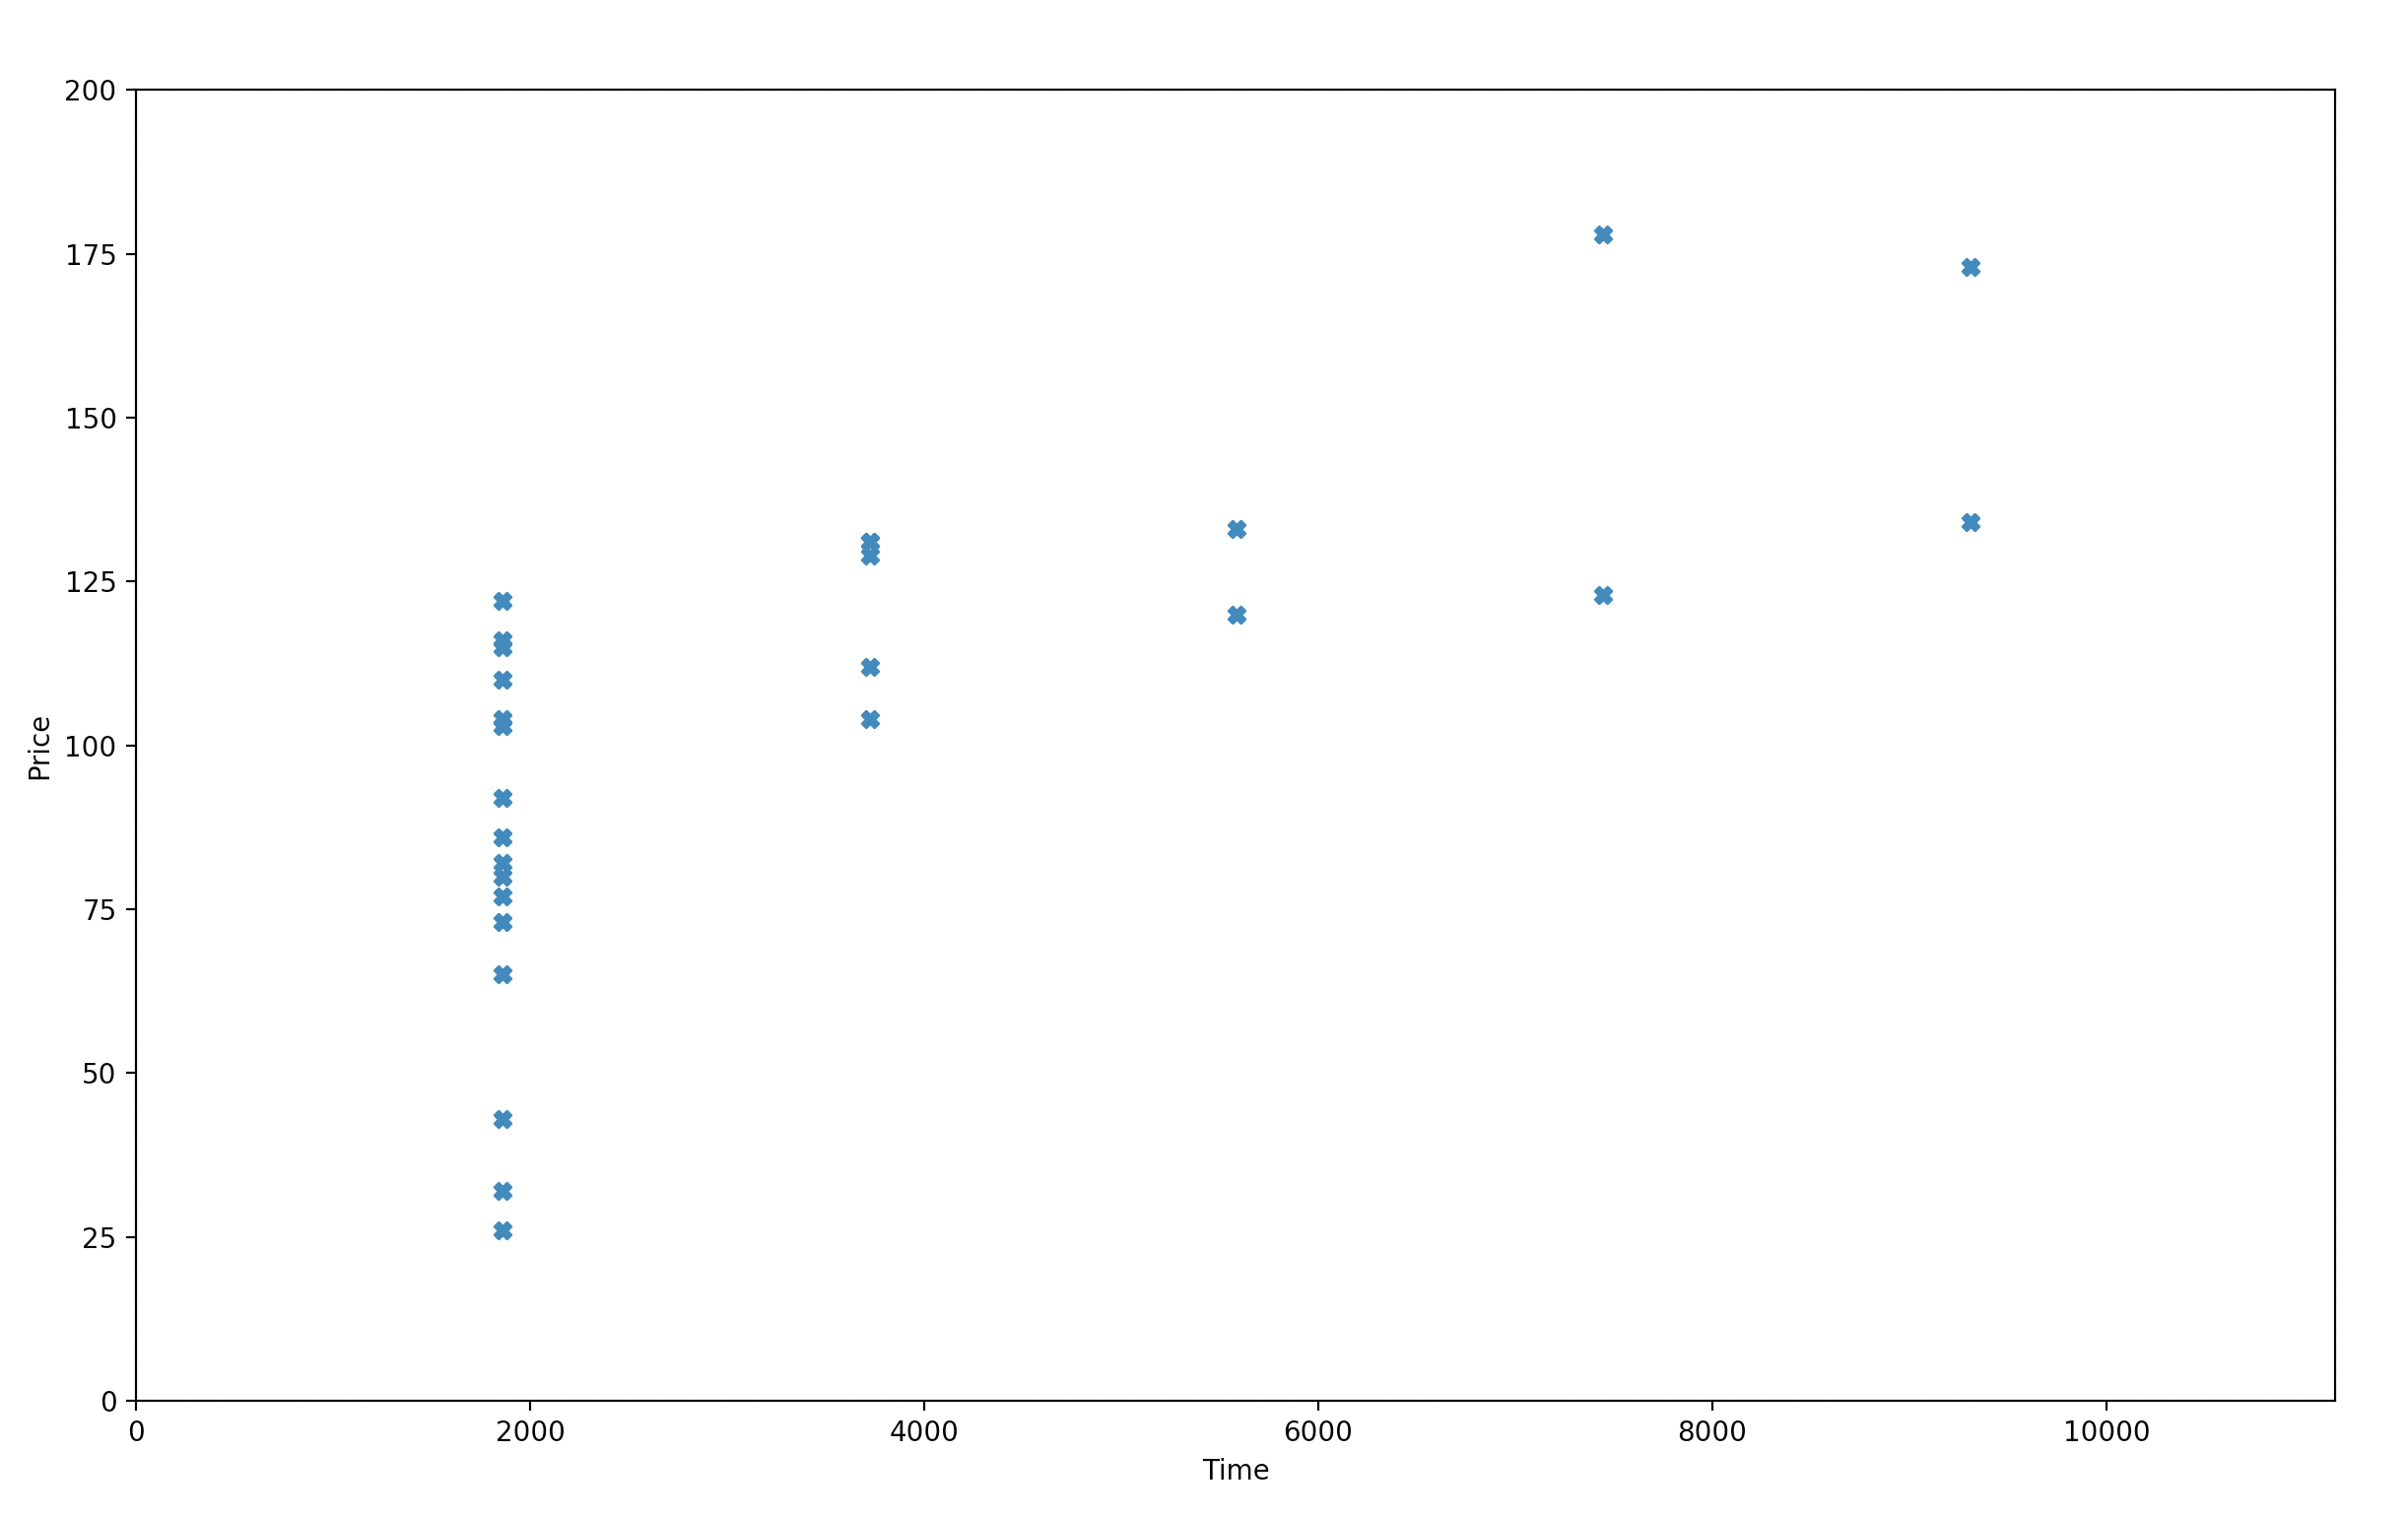
\includegraphics[width=7cm, height=7cm]{Dissertation/images/zip_randomized/1.png}
    \caption{ZI-P with $p_{zip} = 1$ }
    \label{fig:1}
  \end{subfigure}
  %
  \begin{subfigure}[b]{0.5\textwidth}
    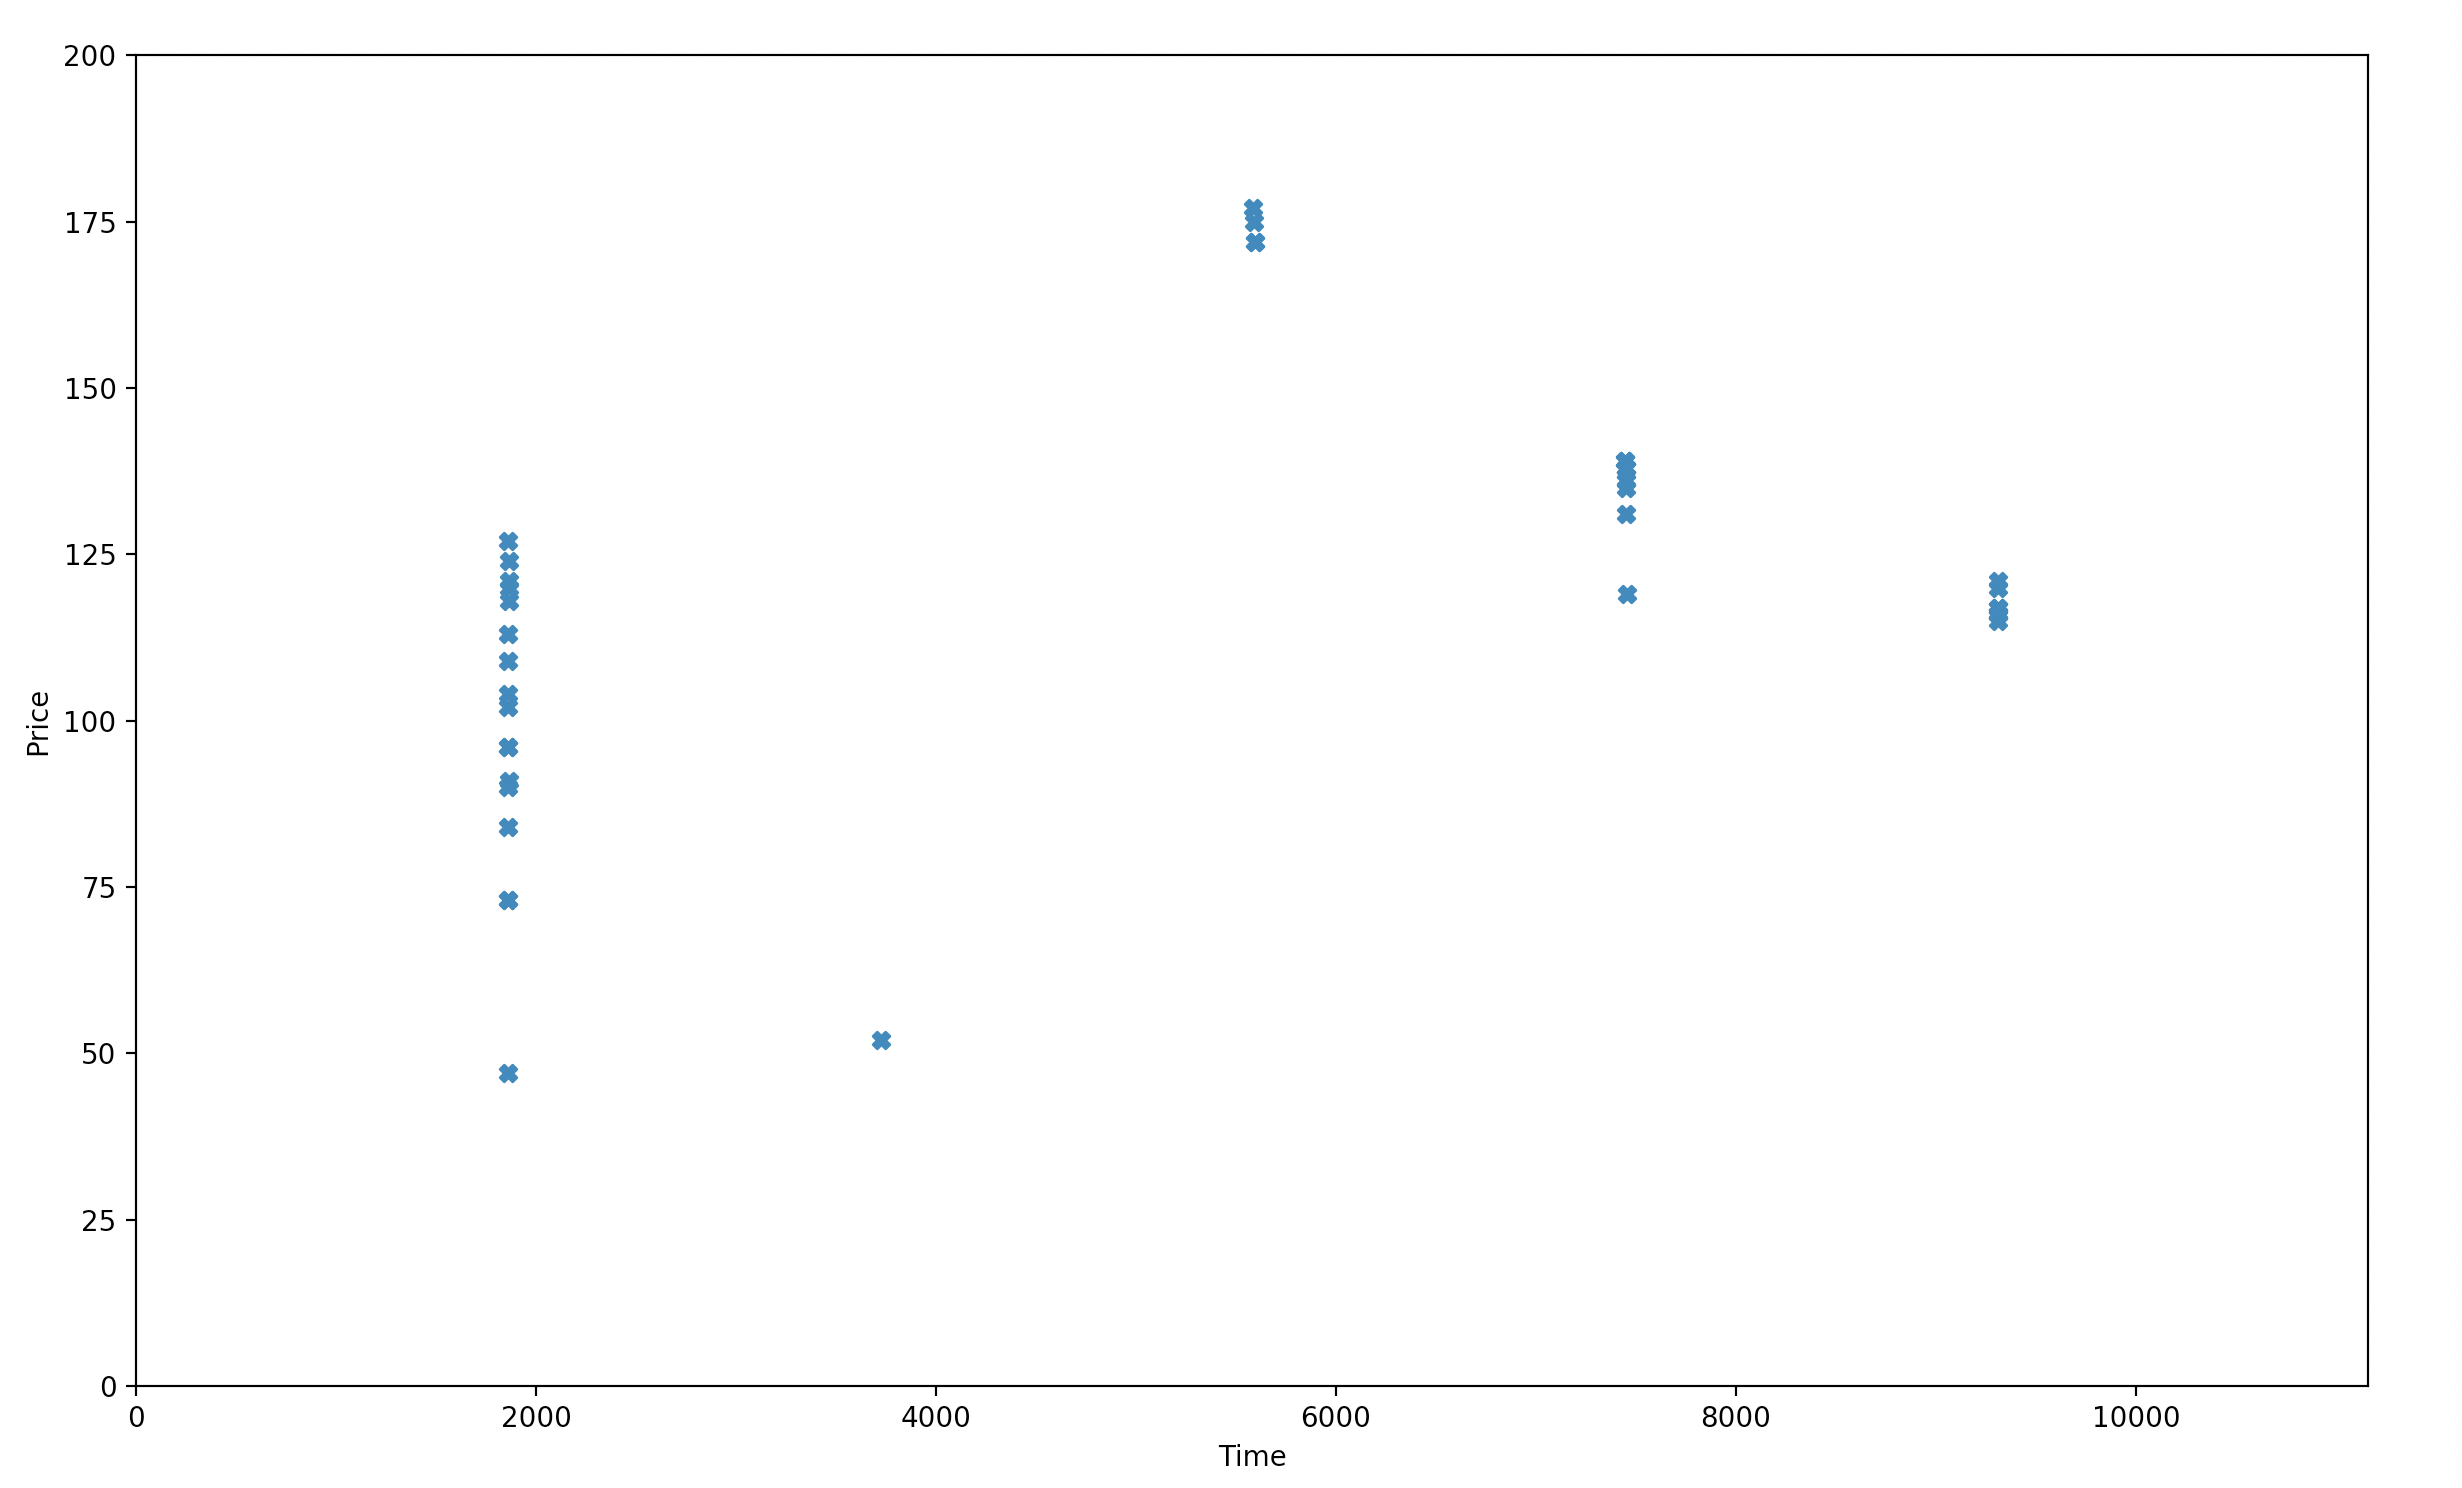
\includegraphics[width= 7cm, height=7cm]{Dissertation/images/zip_randomized/0.5.png}
    \caption{ZI-P with $p_{zip} = 0.5$}
    \label{fig:2}
  \end{subfigure}
\end{figure}

\begin{figure}[h]
  \begin{subfigure}[b]{0.5\textwidth}
    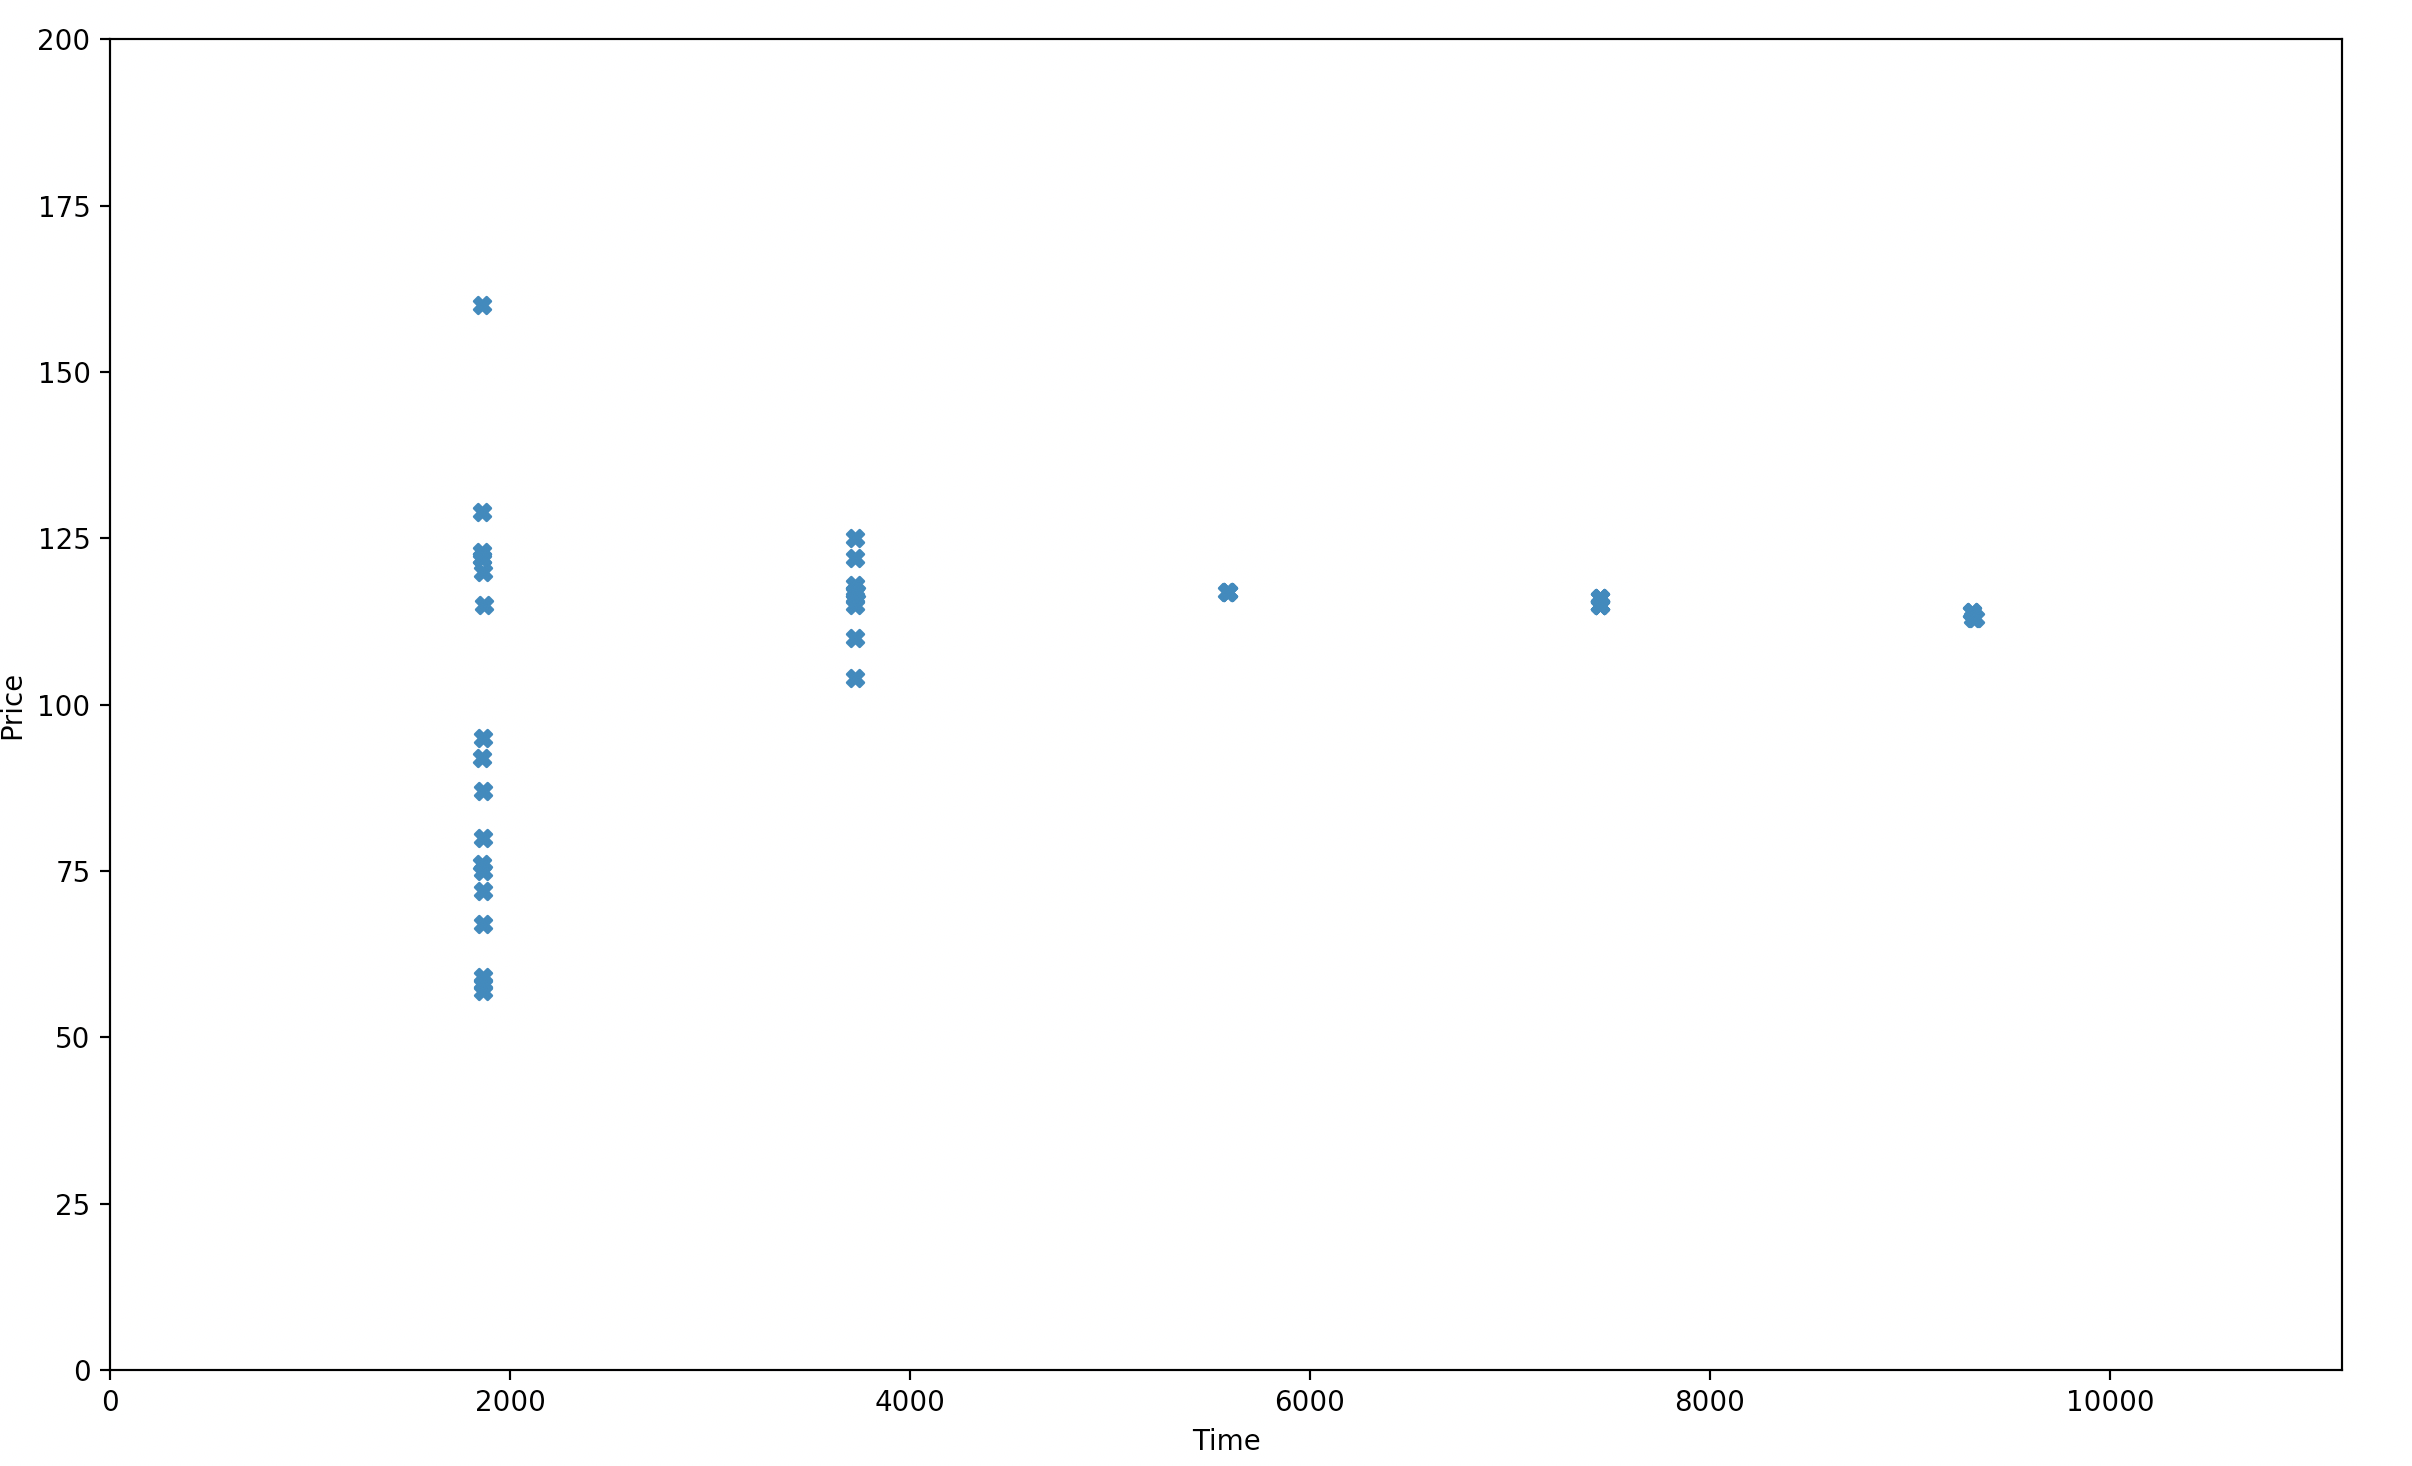
\includegraphics[width= 7cm, height=7cm]{Dissertation/images/zip_randomized/0.25.png}
    \caption{ZI-P with $p_{zip} = 0.25$}
    \label{fig:3}
  \end{subfigure}
  %
  \begin{subfigure}[b]{0.5\textwidth}
    \includegraphics[width= 7cm, height=7cm]{Dissertation/images/change2/zip.png}
    \caption{ZI-P with $p_{zip} = 0.1$}
    \label{fig:4}
  \end{subfigure}
\end{figure}

To illustrate this further, the figures below is the comparison between the final 0.1 probability with the original Base Line ZI-P behaviour. 

\begin{table}[h]
\centering
\begin{tabular}{ |m||p{4cm}|} 
\hline
\textbf{Probability}& \textbf{Smith's alpha value} \\
\hline
\hline
1 & 40.12 \\ 
\hline
0.5 & 41.12\\ 
\hline
0.25 & 32.0 \\ 
\hline
0.1 & 25.4 \\ 
\hline
\end{tabular}
\caption{Smith's alpha value after implementing probability of acting $p_{zip}$}  
\end{table}
\FloatBarrier


\begin{figure}[h]
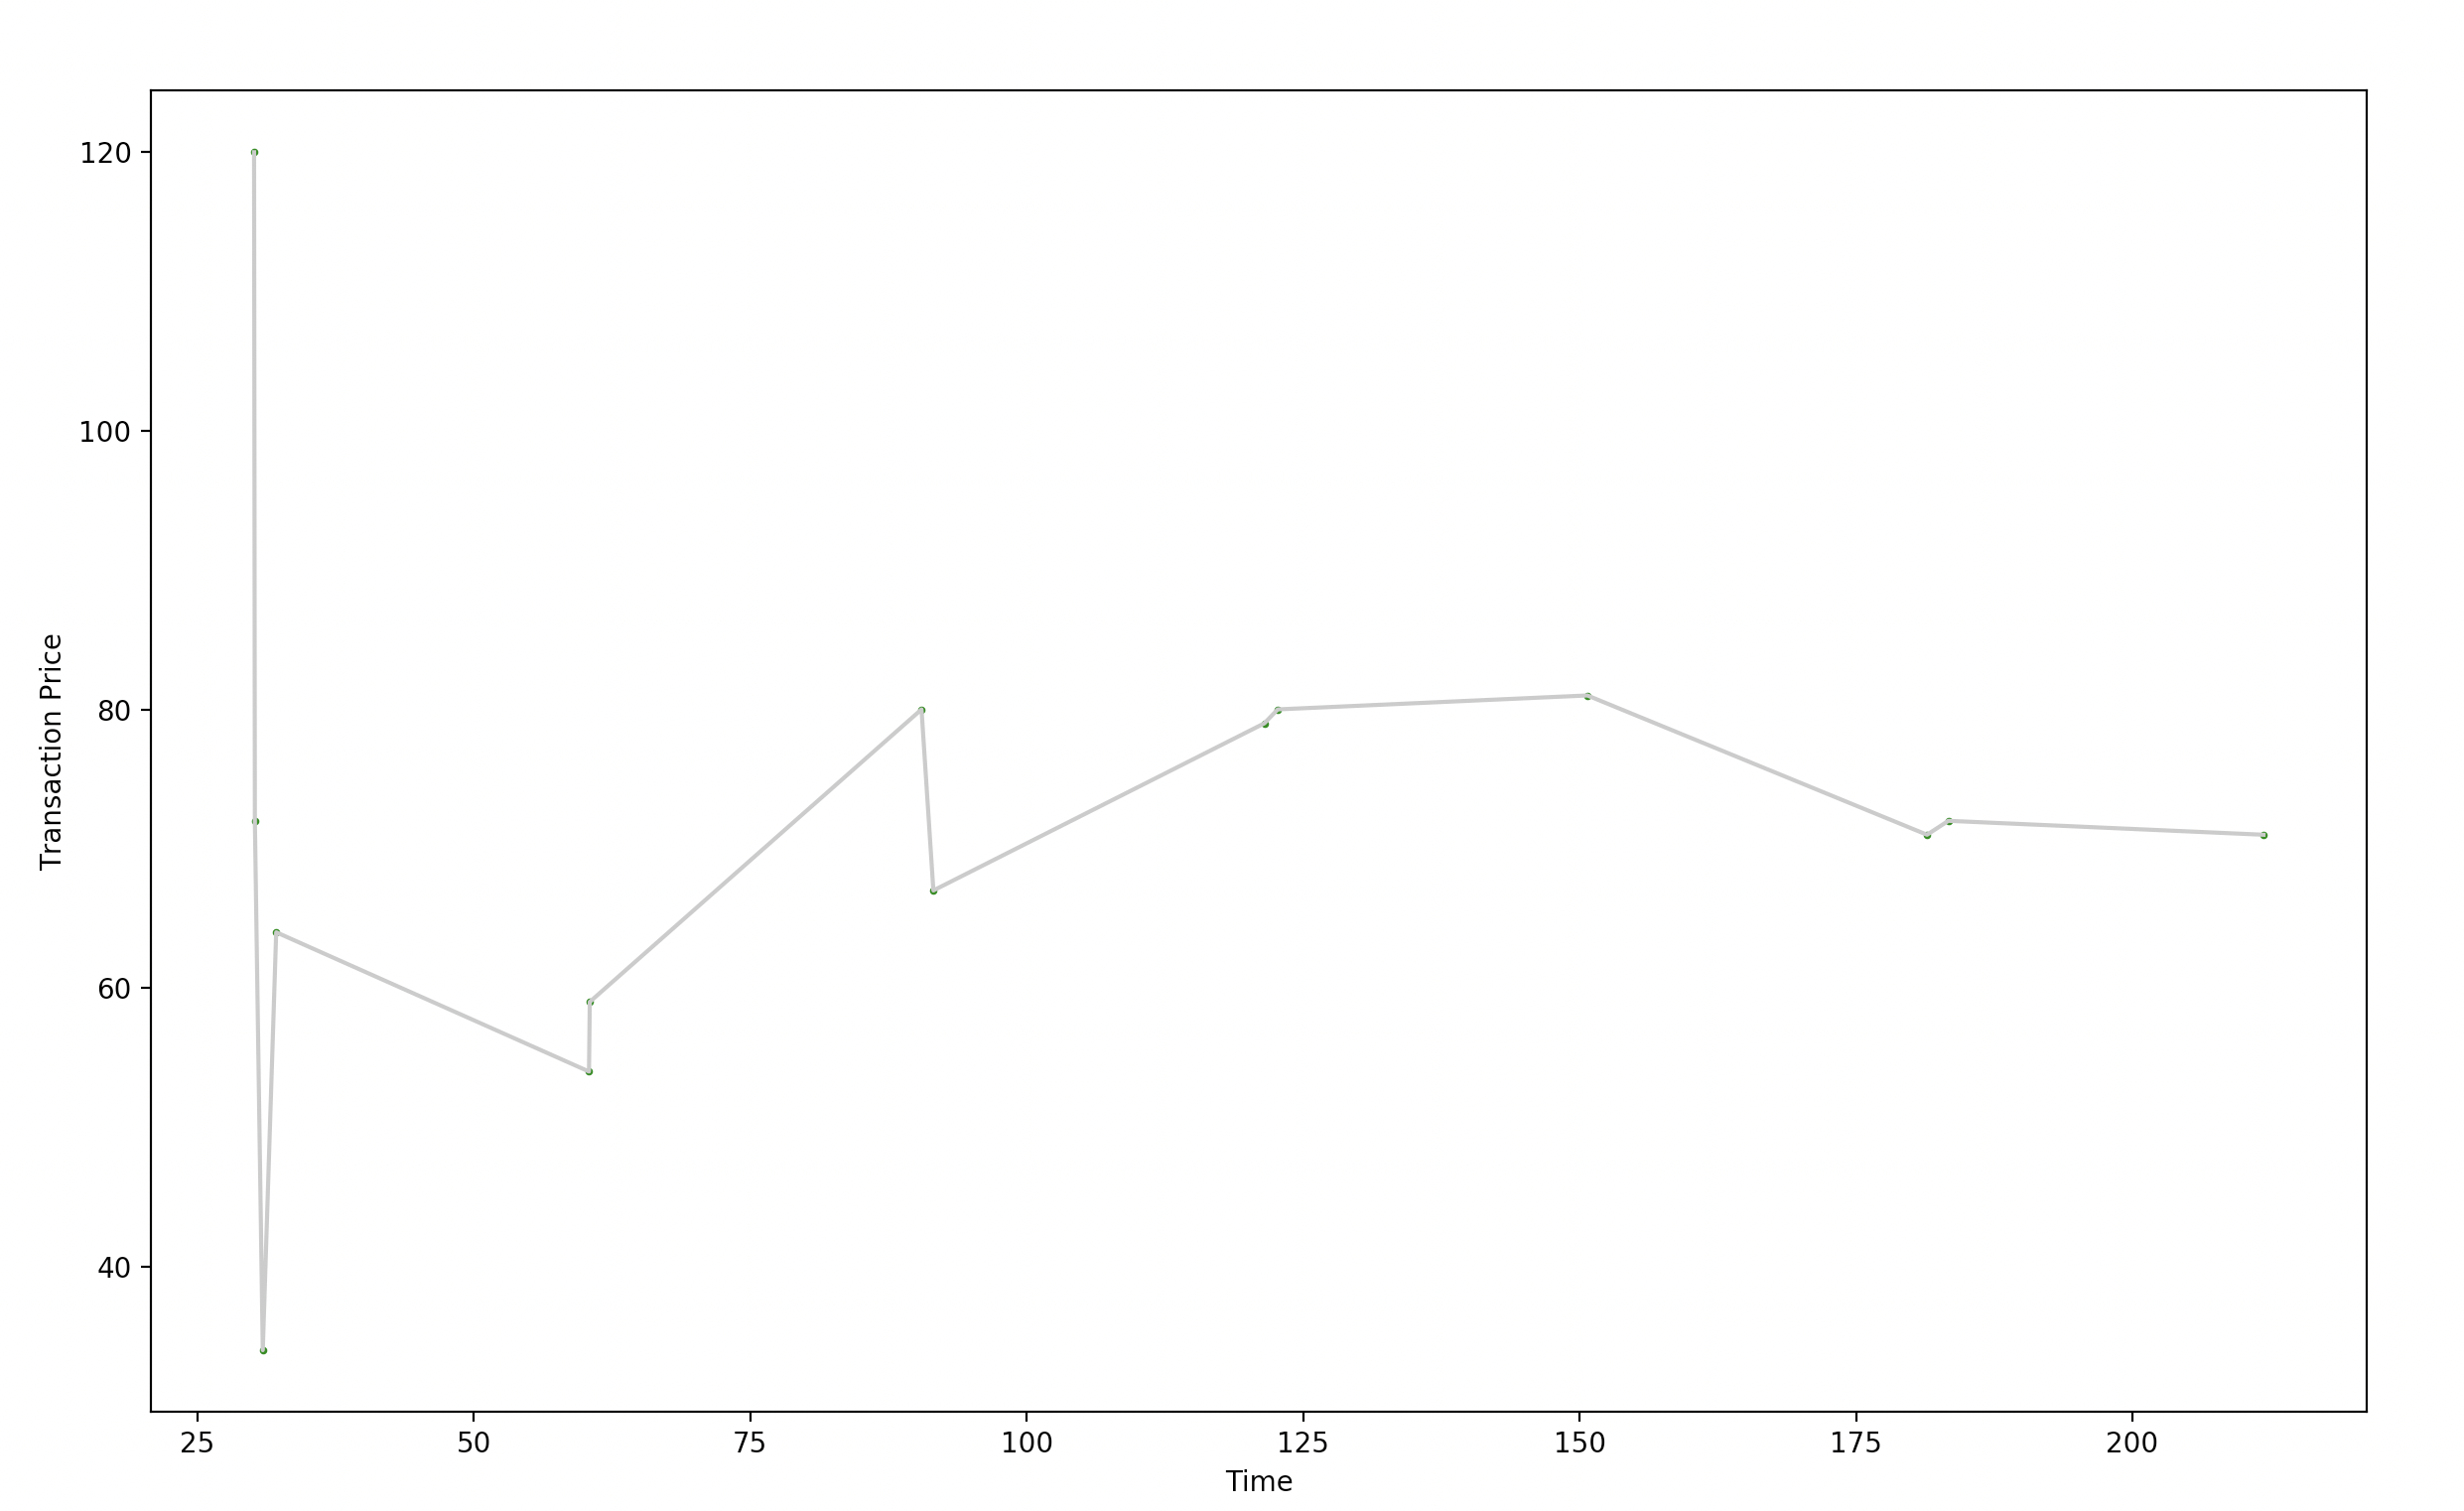
\includegraphics[ height=8cm]{Dissertation/images/base_line/ZIP.png}
\caption{Base Line ZI-P} 
\end{figure} 
\FloatBarrier

\begin{figure}[h]
\includegraphics[ height=8cm]{Dissertation/images/change2/zip.png}
\caption{ZI-P with $p_{zip} = 0.1$} 
\end{figure} 
\FloatBarrier

\section{Number of Transactions}
The table below illustrates the similarities of the number of transactions in each implementation of the BSE.

\begin{table}[h]
\centering
\begin{tabular}{ |m||p{4cm}|p{4cm}|p{4cm}|} 
\hline
\textbf{Agents}& \textbf{Base Line} & \textbf{Section 4.2} & \textbf{McG action step} \\
\hline
\hline
Kaplan's Sniper & 20 & 20 & 20 \\ 
\hline
ZI-C & 71 & 73 & 78\\ 
\hline
ZI-P & 42 & 45 & 47 \\ 
\hline
\end{tabular}
\caption{Number of transactions in each implementation}  
\end{table}
\FloatBarrier